Pada bab ini membahas tentang implementasi metode entropy pada codeigniter, yang dimulai dari perancangan sistem terdiri dari usecase diagram, class diagram, kemudian perancangan database. kemudian setelah itu memulai projek codeigniter dilanjutkan dengan penjelasan dari source code dan penjelasan source code dari logika entropy pada sisitem.
\pagebreak

\section{Perancangan Sistem}
 Adapun perancangan perlu dilakukan di karenakan agar arah dari sistem dapat di ketahui sehingga alur proses atau bisnis proses dari sistem, kemudian selain itu dapat di ketahui sasaran dari sistem yang akan dibuat, maka dari itu pada perancangan sistem ini dilakukan perancangan melaui usecase diagram, class diagram, kemudian perancangan basis data sistem.
Lalu untuk kinerja entropy pada sistem atau logika entropy pada sistem dapat digambarkan pada flowchart berikut ini:\par

\begin{figure}[!htbp]
	\centerline{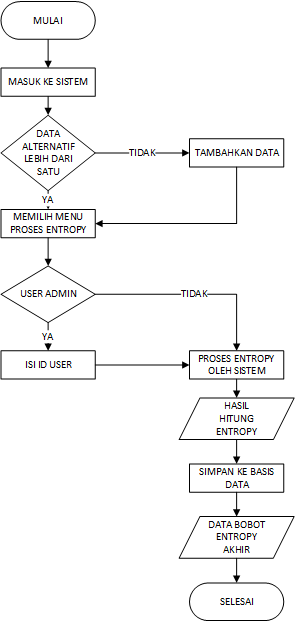
\includegraphics[width=0.50\textwidth]{figures/uml/A.png}}
	\caption{Flowchart Logika Entropy Pada Sistem}
	\label{Flow}
\end{figure}

Pada Folwchart yang terdapat pada gambar \ref{Flow} tersebut dapat di jelaskan menjadi beberapa poin seperti berikut:

\begin{itemize}
\item memuali dengan masuk ke sistem pada tahapan ini telah melalui proses login sistem.
\item Memerikasa data alternatif apakah lebih dari satu atau kurang, jika data kurang maka tambahkan data kemudian lanjutkan keperoses selanjutnya, lalu jika data telah lebih dari 1 (satu) maka lanjutkan ke peroses selanjutnya.
\item memilih menu proses entropy, jika user yang login merupakan user admin maka harus melalui peroses mengisi id user kemudian data baru bisa dilakukan proses entropy, namun jika user yang login buka admin maka ketika memilih menu proses sistem maka sistem akan malakukan proses entropy sesuai dengan user yang login. 
\item setelah itu maka akan muncul hasil dari proses entropy.
\item jika data bobot hasil perhitungan entropy telah muncul maka data dapat di simpan ke basis data sistem
\item Maka databobot dari data alternatif didapatkan.
\end{itemize}
\subsection{Use Case Diagram}
	Pada perancangan sistem ini di butuhkan usecase diagram seperti pada gambar \ref{uml1}, dengan tujuan agar mengetahui peran dari aktor yang terlibat pada sistem, adapun aktor yang terdapat pada sistem ini yaitu aktor admin dan aktor pengambil keputusan

\begin{figure}[!htbp]
	\centerline{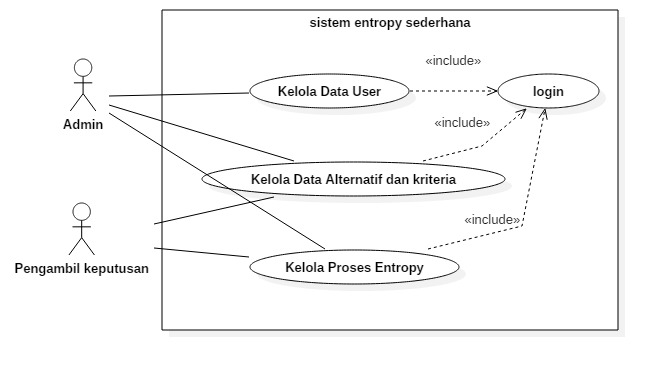
\includegraphics[width=0.90\textwidth]{figures/uml/usecasebuku.jpg}}
	\caption{Use Case Diagram Sistem}
	\label{uml1}
\end{figure}

\pagebreak
\subsection{Class Diagram}
Kemudian setelah membuat usecase diagram dilanjutkan dengan membuat kelas diagram yang bertujuan untuk menunjukan class apa saja dan method apa saja yang digunakan pada sistem untuk class yang di gunakan pada sistem dapat di lihat pada gambar \ref{uml2} berikut ini

\begin{figure}[!htbp]
	\centerline{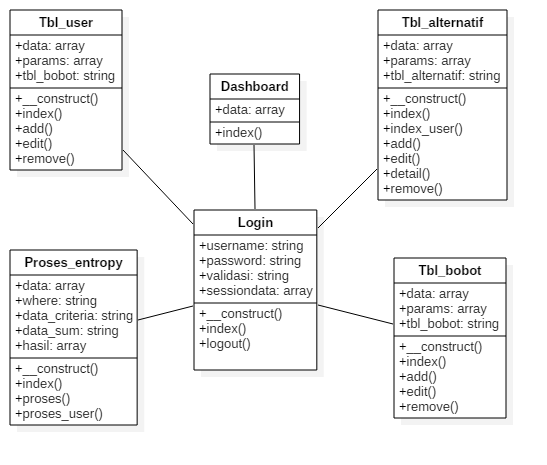
\includegraphics[width=0.90\textwidth]{figures/uml/buku.png}}
	\caption{Class Diagram Sistem}
	\label{uml2}
\end{figure}

\pagebreak
\subsection{Perancangan Basisdata}
Setelah class diagram di buat dilanjutkan dengan membuat perancangan basis data sistem adapun untuk basis data sistem bernama db\_sistem.sql dengan ketentuan tabel-tabel yang terdapat pada basis data tersebut adalah sebagai berikut:

\begin{table}[h]
\caption{User}
\centering
\begin{tabular}{|c|c|c|c|c|}
\hline
 Field Name & Tipe Data & Field Size&Keterangan\\
\hline
user\_id&Int&11&id user (primary key)\\
\hline
user\_name&varchar&20&username user\\
\hline
user\_email&varchar&60&Email user\\
\hline
user\_password&varchar&60&Password user\\
\hline
user\_level&varchar&5&Level user \\
\hline
status &Int&1&Staus user\\
\hline
\end{tabular}
\label{B41}
\end{table}

\begin{table}[h]
\caption{Data Alternatif dan Kriteria}
\centering
\begin{tabular}{|c|c|c|c|c|}
\hline
 Field Name & Tipe Data & Field Size&Keterangan\\
\hline
alternatif\_id&Int&11&id alternatif (primary key)\\
\hline
alternatif\_name&varchar&20&nama dari alternatif\\
\hline
Kriteria\_1l&Int&11&kriteria ke 1\\
\hline
Kriteria\_2&Int&11&kriteria ke 2\\
\hline
Kriteria\_3&Int&11&kriteria ke 3\\
\hline
Kriteria\_4 &Int&11&kriteria ke 4\\
\hline
Id\_user &Int&11&(foregin Key)\\
\hline
\end{tabular}
\label{B42}
\end{table}

\begin{table}[h]
\caption{Data Bobot Entropy}
\centering
\begin{tabular}{|c|c|c|c|c|}
\hline
 Field Name & Tipe Data & Field Size&Keterangan\\
\hline
bobot\_id&Int&11&id bobot (primary key)\\
\hline
Bobot\_kriteria\_1&double&-&Bobot Kriteria ke 1\\
\hline
Bobot\_kriteria\_2&double&-&Bobot Kriteria ke 2\\
\hline
Bobot\_kriteria\_3&double&-&Bobot Kriteria ke 3\\
\hline
Bobot\_kriteria\_4&double&-&Bobot Kriteria ke 4\\
\hline
Id\_user &Int&11&(foregin Key)\\
\hline
\end{tabular}
\label{B41}
\end{table}

\pagebreak
lalu untuk hubungan antara tabel atau relasi antara tabel seperti pada gambar \ref{db1} berikut ini

\begin{figure}[!htbp]
	\centerline{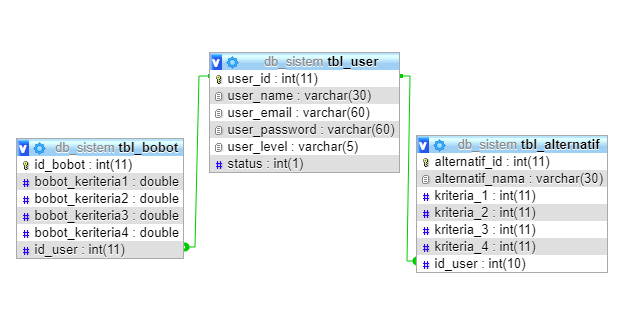
\includegraphics[width=0.90\textwidth]{figures/db/1.png}}
	\caption{Relasi Antara Tabel Pada Basis Data Sistem}
	\label{db1}
\end{figure}

pada gambar \ref{db1} tersebut merupakan gambar relasi antara tabel, dimana tabel yang di gunakan terdiri dari tiga tabel yaitu tabel user, tabel bobot, dan tabel alternatif, dimana untuk menghubungkan ke tiga tabel tersebut menggunakan id user yang di jadi kan tiga kunci yaitu primarry key dan foregin key pada tabel bobot dan tabel alternatif. Kemudian untuk merelasikan tabel seperti pada gambar \ref{db1} tersebut terdapat beberapa tahapan diantaranya:
\begin{enumerate}
\item berikan index pada kolom tabel yang akan di jadikan foregin key untuk contoh pemberian indeks pada kolom tabel atau pada field, dapat dilakukan dengan cara buka phpmyadmin kemudian pilih tabel yang akan di berikan indeks, setelah itu pilih lainnya dan terakhir klik index. maka pada tabel akan muncul tanda kunci, untuk detailnya seperti pada gambar \ref{db2}.

\item jika telah selesai memberikan indeks pada keseruluhan tabel yang akan di relasikan, pada phpmyadmin masuk ke database yang akan di buat relasi antara tabelnya kemudian pilih designer setelah itu jika telah masuk ke halamaman designer pilih create relationship, kemudian pilih kunci rujukan dan kunci foregin key.
\end{enumerate}
\pagebreak

\begin{figure}[!htbp]
	\centerline{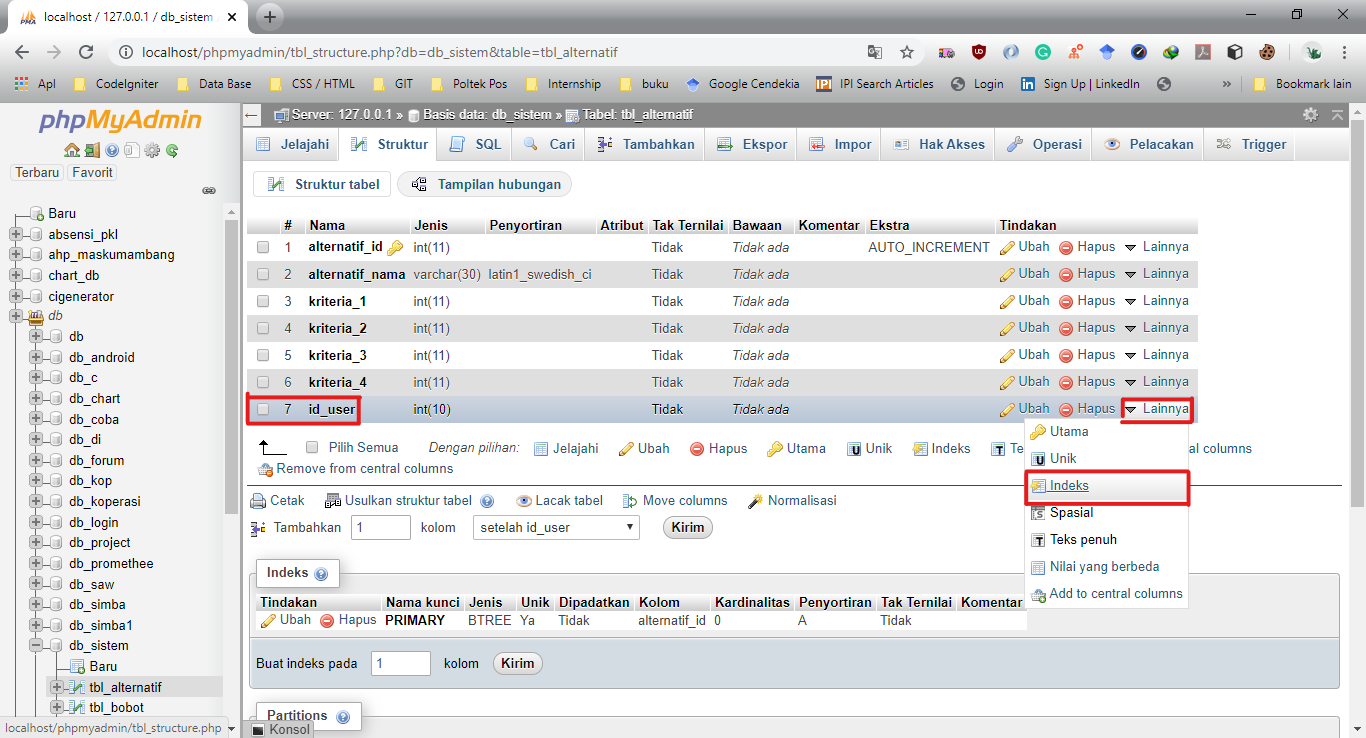
\includegraphics[width=0.90\textwidth]{figures/db/2.png}}
	\caption{Contoh Memberikan Indeks Pada Tabel User}
	\label{db2}
\end{figure}

	Pada gambar tersebut merupakan contoh untuk memberikan indeks pada satu kolom yang terdapat pada tabel dengan cara pilih kolom yang akan di jadikan foregin key kemudian pilih menu lainnya selanjutnya klik index, jika muncul popup pemberitahuna pilih ok, adapun alternatif lain untuk memberikan indeks pada suatu tabel yaitu dengan menggunaka query seperti berikut:\par

\begin{verbatim}
ALTER TABLE `nama_tebel` ADD INDEX(`nama kolom`);
\end{verbatim}

Jika telah di berikan indeks pada kolom tersebut maka akan muncul tanda kinci bewarna abu-abu seperti pada gambar \ref{db3} berikut:

\begin{figure}[!htbp]
	\centerline{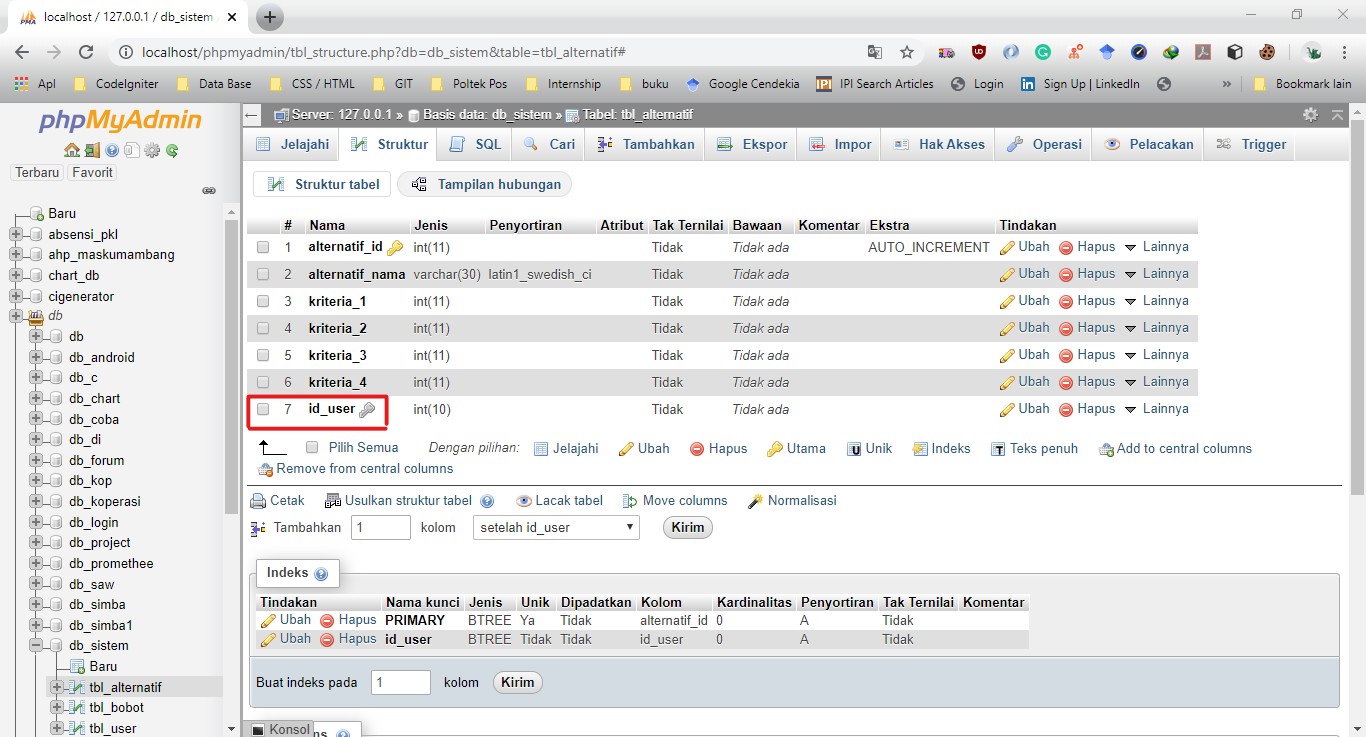
\includegraphics[width=0.90\textwidth]{figures/db/3.png}}
	\caption{Hasil Memberikan Indeks Pada Tabel Alternatif}
	\label{db3}
\end{figure}
\pagebreak

adapun untuk memberikan index pada tabel yang lainnya proses dan langkanya juga sama seperti pada tabel alternatif dan tabel user sehingga hasil pemberian indeks pada tabel bobot seperti pada gambar \ref{db4}


\begin{figure}[!htbp]
	\centerline{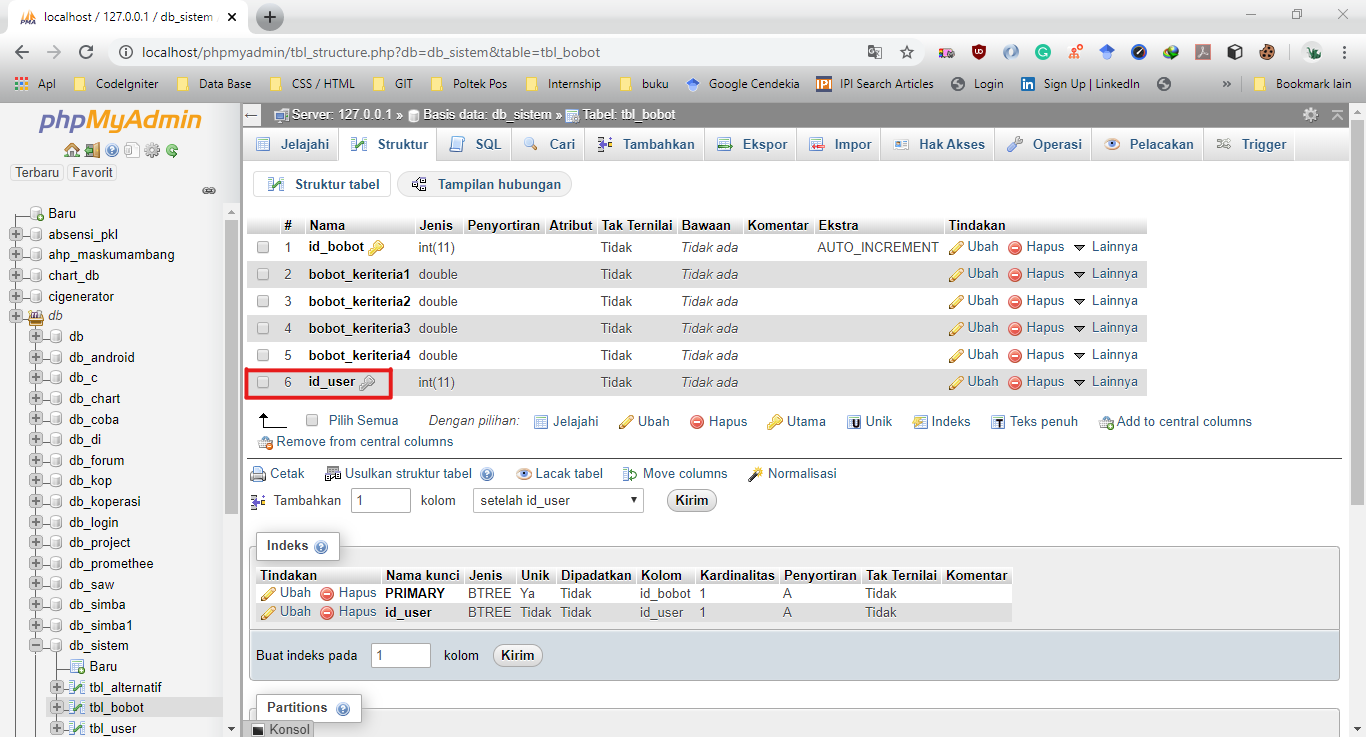
\includegraphics[width=0.90\textwidth]{figures/db/4.png}}
	\caption{Hasil Memberikan Indeks Pada Tabel Bobot}
	\label{db4}
\end{figure}

kemudian untuk menghubungkan tabel, seperti yang telah di jelaskan pada tahap ke dua sebelumnya yaitu dengan mengklik lainnya pada menu database di phpmyadmin kemudian pilih lainnya dan pilih designer, untuk lebih jelasnya seperti pada gambar \ref{db5} berikut ini:

\begin{figure}[!htbp]
	\centerline{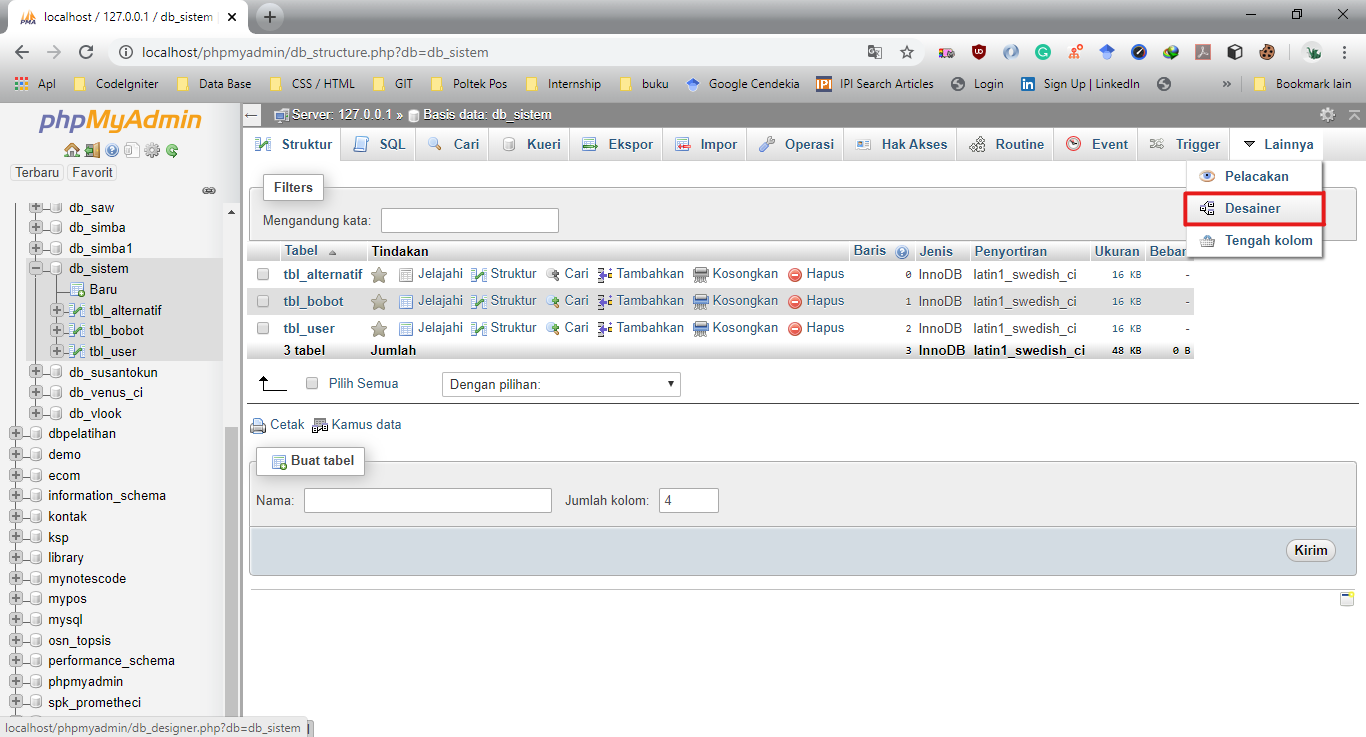
\includegraphics[width=0.90\textwidth]{figures/db/5.png}}
	\caption{Memilih Menu Designer }
	\label{db5}
\end{figure}

Setelah itu jika telah masuk ke menu designer pilih menu relationship seperti pada gambar \ref{db6} berikut ini:
\begin{figure}[!htbp]
	\centerline{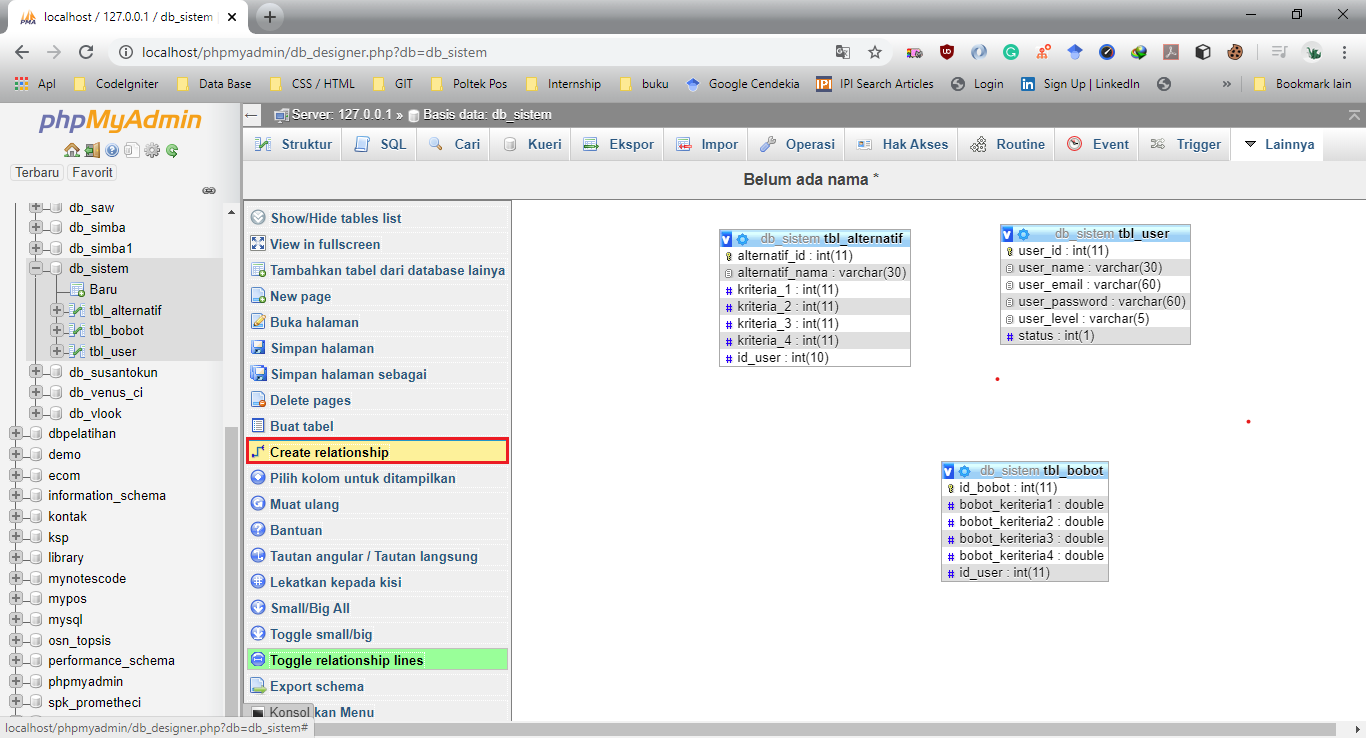
\includegraphics[width=0.90\textwidth]{figures/db/6.png}}
	\caption{Memilih Menu Relationship}
	\label{db6}
\end{figure}

jika telah memilih menu create relationship pilih kunci rujukan yaitu user\_id pada tabel user kemudian klik id\_user pada tabel alternatif begitu pula prosesnya untuk menghubungkan tabel user dengan tabel bobot. Sehingga hasilnya akan seperti pada gambar \ref{db7} berikut ini:
\begin{figure}[!htbp]
	\centerline{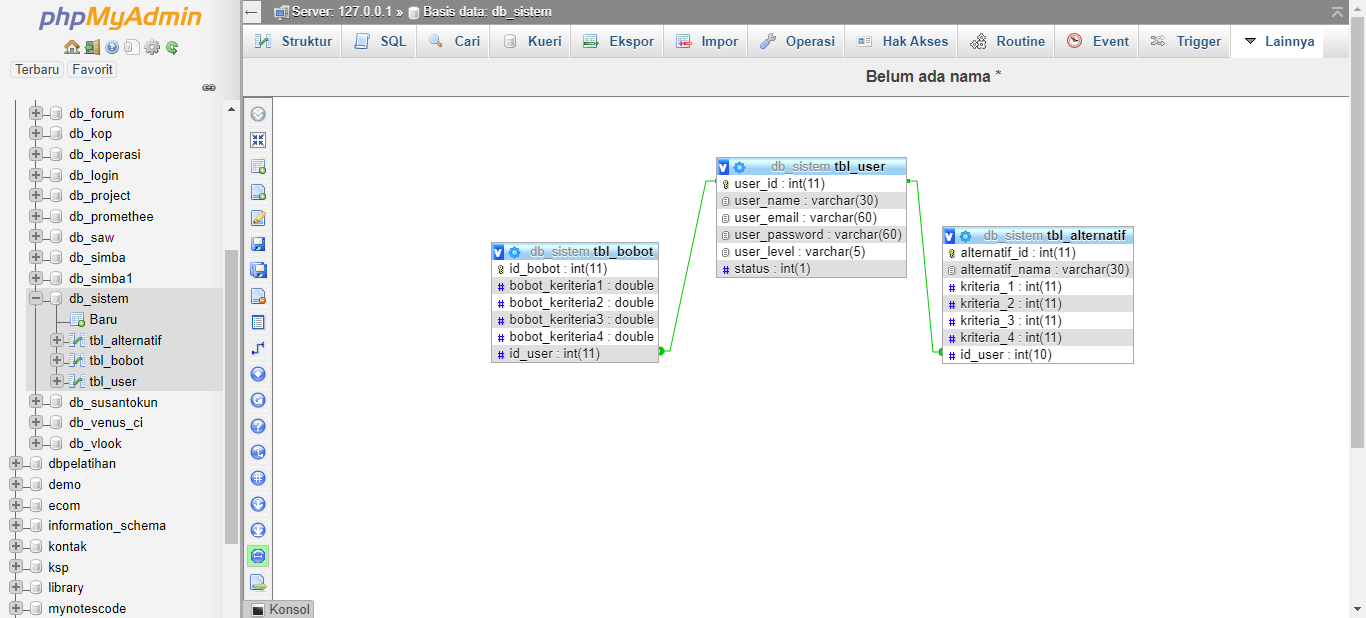
\includegraphics[width=0.90\textwidth]{figures/db/7.png}}
	\caption{hasil relasi antara tabel}
	\label{db7}
\end{figure}
pada gambar \ref{db7} tersebut terlihat garis antara tabel dan menunjuk pada setiap kolom id\_user yang berarti setiap tabel tersebut telah berrelasi.

\textbf{Catatan :}\par
\textit{Jika tabel telah di relasikan berarti tabel tersebut akan saling melengkapi, tidak bisa berdiri sendiri, sehingga jika satu tabel kosong maka bisa kemungkinan akan terjadi error, agar menghindari hal tersebut pada kasus ini tabel yang wajib di isi terlebih dahulu merupakan tabel user, dikarenakan id user terbawa ke seruruh tabel yang terdapat pada basis data sistem.} 

\pagebreak
\section{Pembuatan Sistem Entropy}

Untuk persiapan pembuatan sistem entropy diantaranya yaitu :
\begin{enumerate}
\item Codeigniter versi 3
\item Web server local (yang terinstall pada computer)
\item code editor (direkomendasikan menggunakan visual studio code dengan ketentuan seperti pada bab 1 buku ini)
\end{enumerate}
	Setelah selesai membuat database dilanjutkan dengan instalisasi codeigniter yaitu dengan cara download terlebih dahulu codeigniter pada situs resminya. Hal ini dapat mengikuti langkah langkah pada bab1 namun untuk nama projeknya di ganti menjadi projek\_entropy sehingga pada htdocs tampilannya seperti pada gambar \ref{crs1} berikut.

\begin{figure}[!htbp]
	\centerline{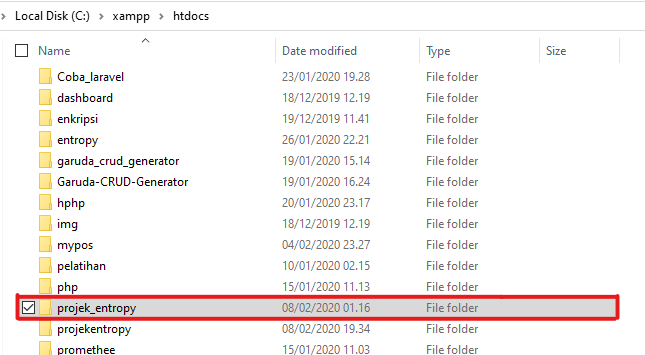
\includegraphics[width=0.90\textwidth]{figures/crs/1.png}}
	\caption{hasil relasi antara tabel}
	\label{crs1}
\end{figure}

jika telah folder codeigniter telah disimpan pada htdocs seperti pada gambar \ref{crs1} tersebut lanjutkan dengan melakukan konfigurasi, adapun file yang harus di lakukan konfigurasi yaitu pada file berikut:

\begin{itemize}
\item file config.php
\item file autoload.php
\item file database.php
\end{itemize}
\pagebreak
kemudian untuk tempat file serta source code yang harus di ubah adalah sebagai berikut:

\begin{itemize}
\item C:/xampp/htdocs/projekentropy/application/config/autoload.php kemudian source code yang harus di ubah yaitu
\begin{lstlisting}[language=PHP]
$autoload['libraries'] = array('database', 'pagination');
$autoload['helper'] = array('security','form','url');
\end{lstlisting} 
\item C:/xampp/htdocs/projekentropy/application/config/config.php kemudian source code yang harus di ubah yaitu
\begin{lstlisting}[language=PHP]
$config['base_url'] = 'http://localhost/projek_entropy//';
\end{lstlisting}
\item C:/xampp/htdocs/projekentropy/application/config/database.php kemudian source code yang harus di ubah yaitu
\begin{lstlisting}[language=PHP]
$active_group = 'default';
$query_builder = TRUE;

$db['default'] = array(
	'dsn'	=> '',
	'hostname' => 'localhost',
	'username' => 'root',
	'password' => '',
	'database' => 'db_sistem',
	'dbdriver' => 'mysqli',
	'dbprefix' => '',
	'pconnect' => FALSE,
	'db_debug' => (ENVIRONMENT !== 'production'),
	'cache_on' => FALSE,
	'cachedir' => '',
	'char_set' => 'utf8',
	'dbcollat' => 'utf8_general_ci',
	'swap_pre' => '',
	'encrypt' => FALSE,
	'compress' => FALSE,
	'stricton' => FALSE,
	'failover' => array(),
	'save_queries' => TRUE
);

\end{lstlisting}
\end{itemize}
\pagebreak
Kemudian pada direktori utama codeigniter akan di tambahkan file bernama .htaccess yang berguna untuk menghilangkan penulisan index.php pada alamat codeigniter, misalkan yang awalnya http://codeigniter/index.php/controller/ menjadi \\
http://codeigniter/controller/ saja tetapi masih menghasilkan tampilan yang sama. Untuk menerapkan file .htaccess dapat dilakukan dengan cara mengakses dokumentasi codeigniter baik online maupun bawaan dari codeigniter itu sendiri untuk tampilan dari dokumentasi codeigniter seperti pada gambar \ref{crs2} berikut:\par


\begin{figure}[!htbp]
	\centerline{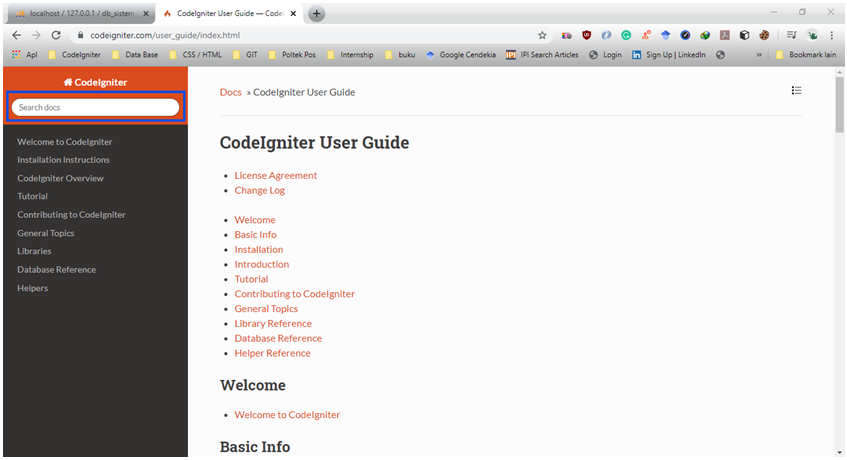
\includegraphics[width=0.90\textwidth]{figures/crs/2.png}}
	\caption{Dokumentasi Codeigniter}
	\label{crs2}
\end{figure}


Setelah mendapatkan tampilan seperti pada gambar \ref{crs2} pada browser kemudian pada menu pencharian ketik index kemudian tekan enter, sehingga akan muncul tampilan seperti pada gambar \ref{crs3} berikut \par

\begin{figure}[!htbp]
	\centerline{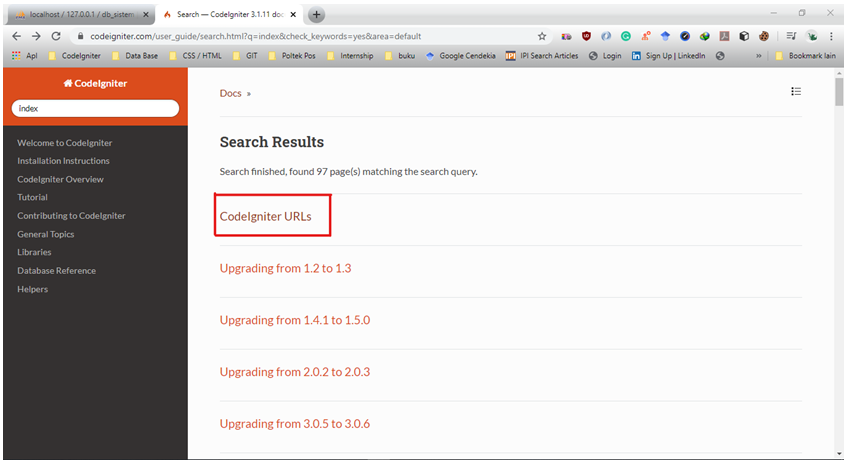
\includegraphics[width=0.90\textwidth]{figures/crs/3.png}}
	\caption{Hasil Pencarian}
	\label{crs3}
\end{figure}
\pagebreak
Pada gambar berikut pilih CodeIgniter URLs kemudian gulung ke bawah dan carai codingan removing index.php seperti pada gambar \ref{crs4} setelah itu copy code tersebut dan masukan pada file .htaccess pada direktori utama codeigniter kemudian save, maka index.php pada codeigniter telah di hilangkan,

\begin{figure}[!htbp]
	\centerline{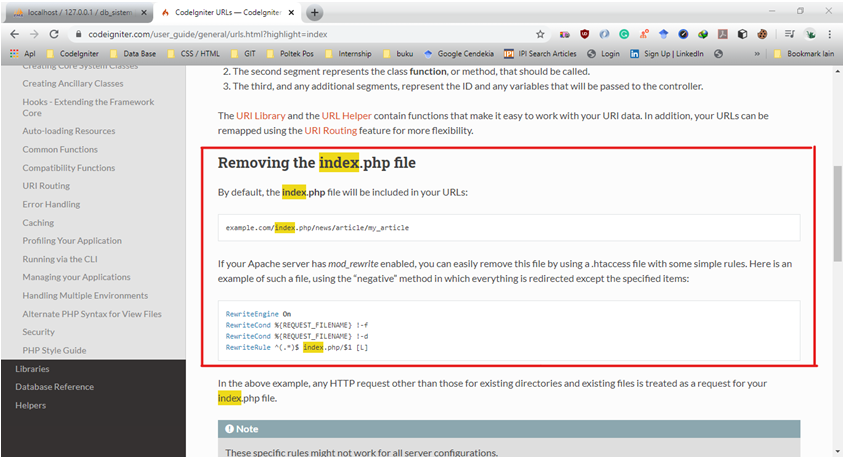
\includegraphics[width=0.90\textwidth]{figures/crs/4.png}}
	\caption{Code Removing index.php}
	\label{crs4}
\end{figure}

adapun penempatan file ht akses pada direktori utama projek\_entropy seperti pada gambar \ref{crs5} berikut ini.

\begin{figure}[!htbp]
	\centerline{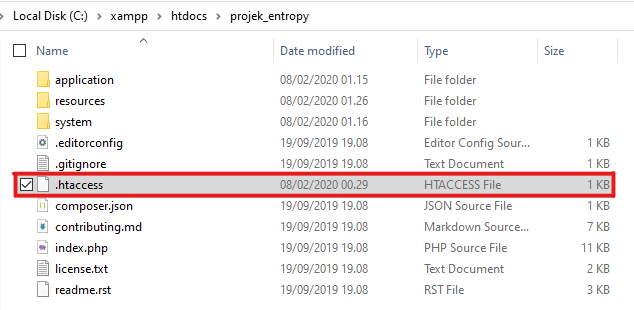
\includegraphics[width=0.90\textwidth]{figures/crs/5.png}}
	\caption{Tempat Direktori .htaccess disimpan}
	\label{crs5}
\end{figure}

\pagebreak
\subsection{Penggunaan template}

pada pembuatan sistem ini untuk tampilan itu sendiri menggunakan template, template itu sendiri agar memperindah tampilan dari sistem itu sendiri, selain memperindah tampilan dengan menggunakan template seorang programmer tidak usah membuat tampilan dari awal, tinggal menggunakan template sesuai dengan kebutuhan.\par
	kemudian untuk implementasi sistem ini dalam penmbuatannya menggunakan template Admin LTE, yang merupakan Template css yang telah umum di gunakan, untuk penggunaannya penulis menggunakan template Admin LTE versi 3 yang telah di dukung oleh css bootstrap 4 dan library terbaru dari css dan java script, untuk template Admin LTE sendiri dapat di download pada website resminya yaitu https://adminlte.io/ atau pada alamat\\ github berikut https://github.com/ColorlibHQ/AdminLTE.
	lalu jika menggunakan github alangkah baiknya menggunakan git scm sebagai alat untuk mendownload data dari github, namun jika git scm tidak terinstall pada computer maka alternatifnya yaitu mendownload file zip dari github.
untuk caranya yaitu :
\begin{itemize}
\item pertama buka link github dari Admin LTE 
\item Kemudian jika telah muncul halaman Admin LTE tekan clone dan download 
\item langkah terakhir tekan Downliad ZIP 
\end{itemize}

untuk lebih jelasnya dapat di lihat pada gambar \ref{tmp1} berikut ini:

\begin{figure}[!htbp]
	\centerline{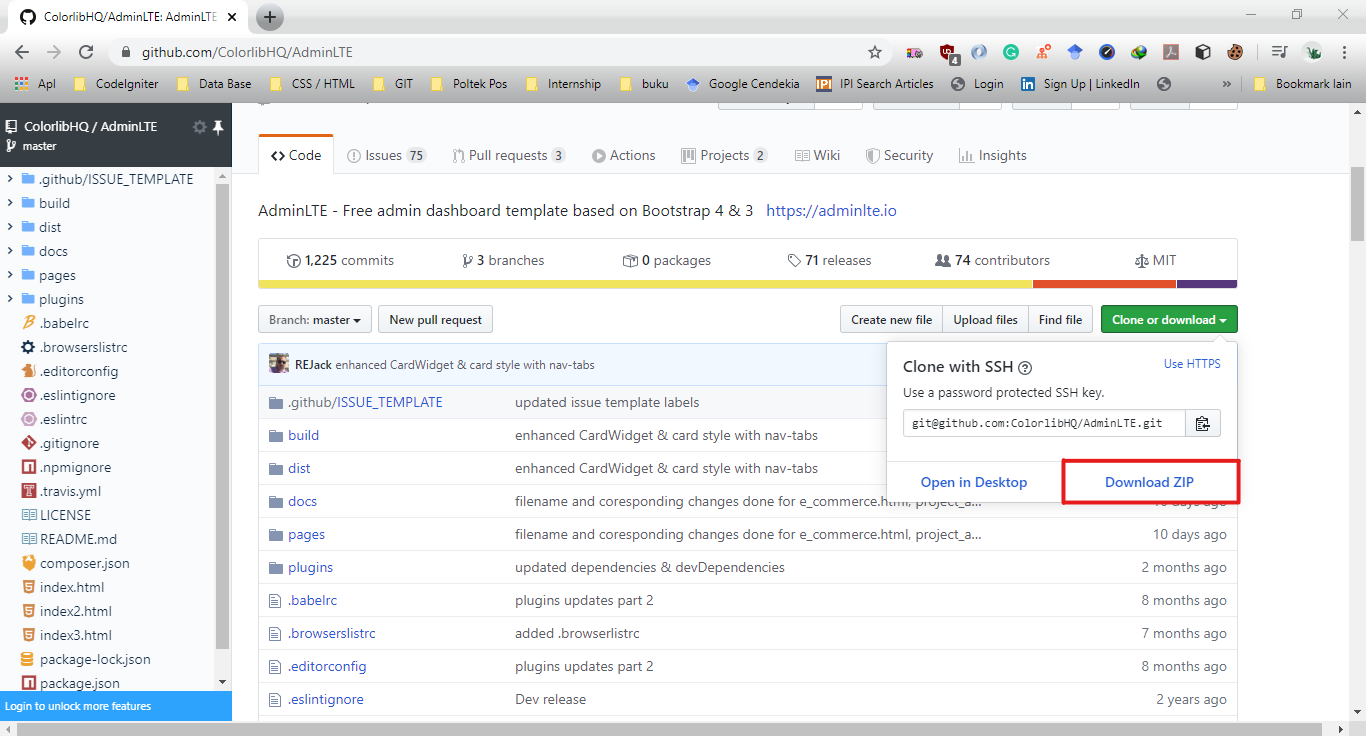
\includegraphics[width=0.90\textwidth]{figures/tmp/1.png}}
	\caption{Halaman Website Git Untuk Template Admin LTE}
	\label{tmp1}
\end{figure}
\pagebreak

Setelah file tempalate di unduh ekstrak terlebih dahulu file tersebut kemudian filih folder dist dan folder plugins, kemudian buka folder dist lalu copy semu folder dan file yang terdapat pada folder tersebut dan pindahkan ke folder resources pada direktory projek\_entropy, kemudian dilanjutkan dengan memindahkan folder css dan js yang terdapat pada folder plugins, yang akan di gunakan dalam projek atau jika tidak mau ribet bisa di copy semua folder css dan js yang terdapat pada folder fligins kemudian pindahkan ke folder resources. agar lebih jelas tempat dari kedua folder yang di pendahkan yaitu terdapat pada direktori utama Admin LTE-master seperti pada gambar \ref{tmp2} berikut ini.

\begin{figure}[!htbp]
	\centerline{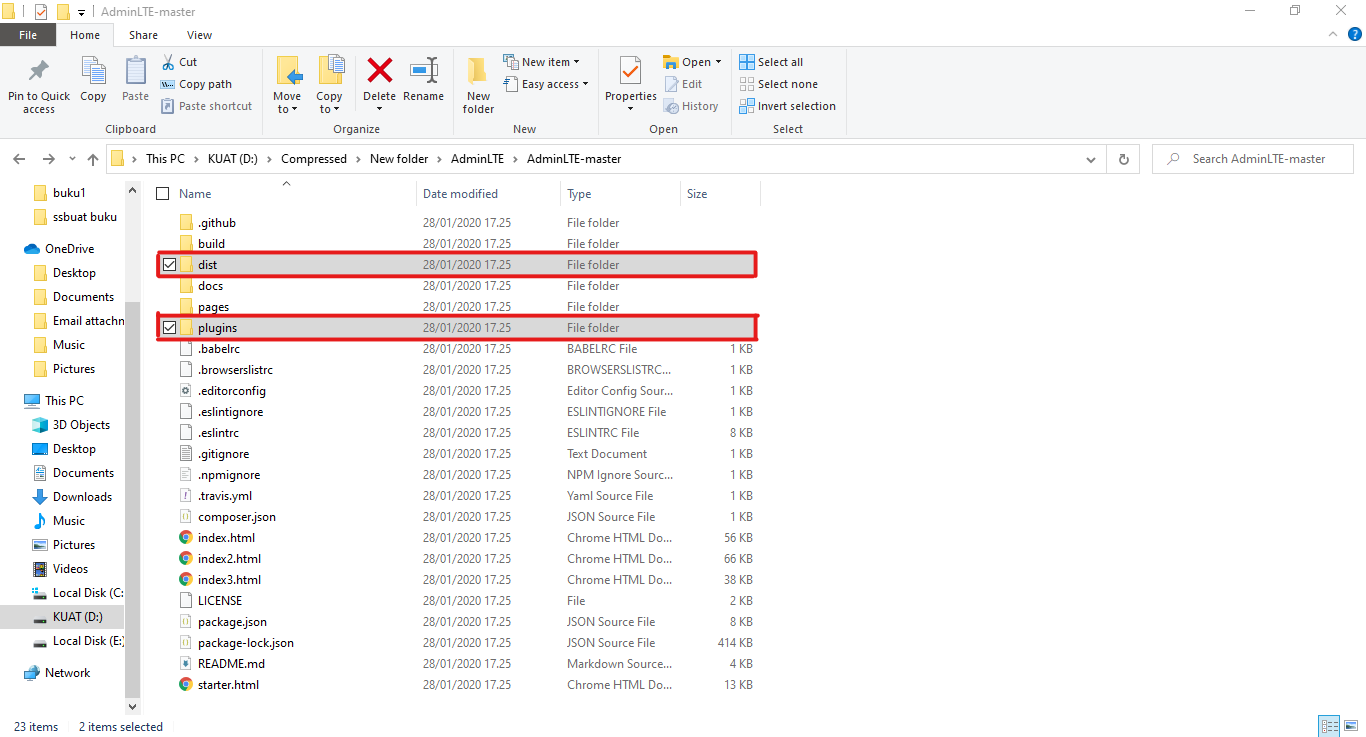
\includegraphics[width=0.90\textwidth]{figures/tmp/2.png}}
	\caption{Direktori Utama Admin LTE=master}
	\label{tmp2}
\end{figure}

setelah di pindahkan ke folder resource maka hasilnya seperti pada gambar \ref{tmp3} berikut:

\begin{figure}[!htbp]
	\centerline{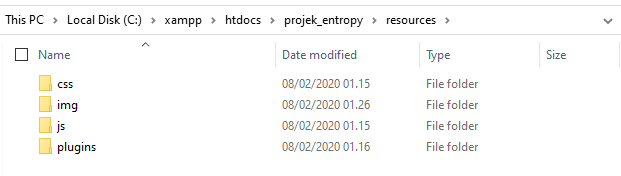
\includegraphics[width=0.90\textwidth]{figures/tmp/3.png}}
	\caption{Folder Yang di pindahkan}
	\label{tmp3}
\end{figure}
	
\pagebreak
Setelah itu buat folder layout pada folder views pada subdirektori application pada direktori projek\_entropy kemudian isi dengan file main.php jelasnya seperti pada gambar \ref{tmp4} berikut ini.

\begin{figure}[!htbp]
	\centerline{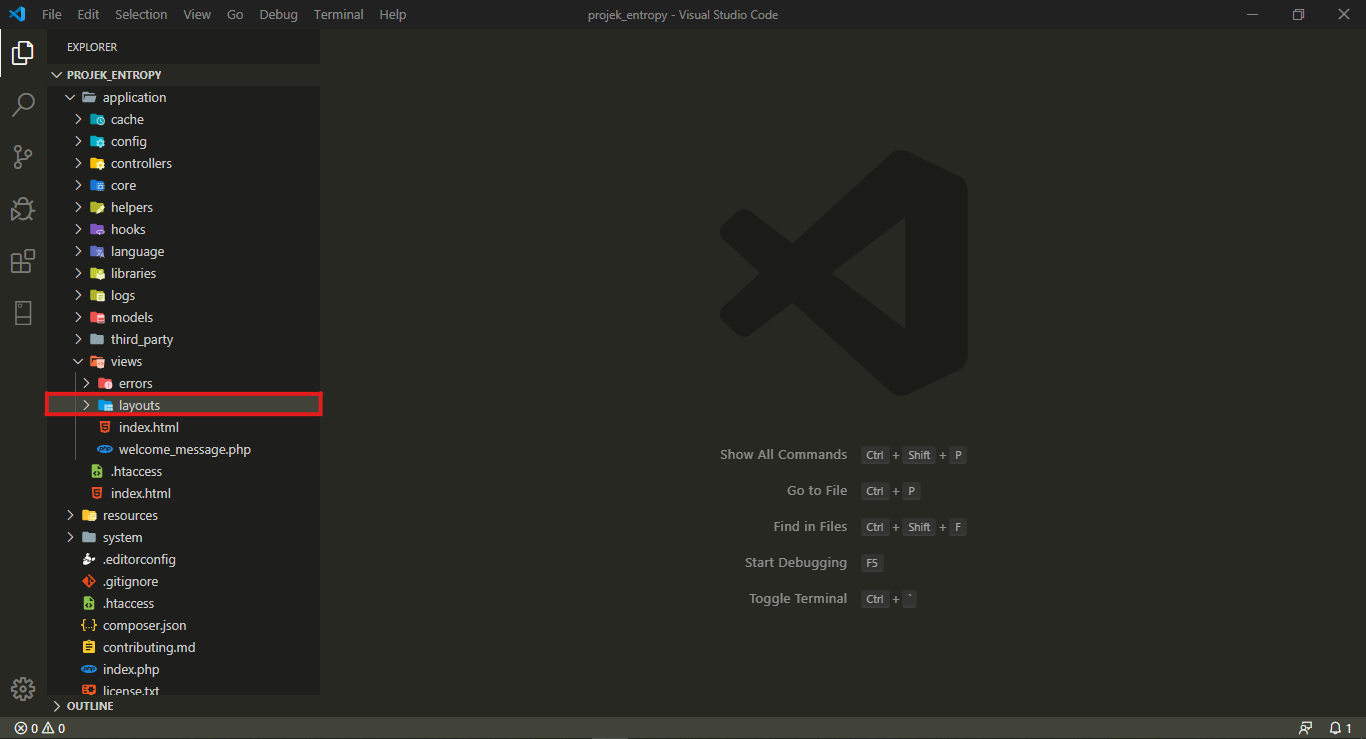
\includegraphics[width=0.90\textwidth]{figures/tmp/6.png}}
	\caption{File main.php pada view}
	\label{tmp4}
\end{figure}

setelah file main.php telah di buat buka file index.html yang terdapat pada direktori AdminLTE-master menggunakan visual stidio code kemudian copy semua code yang terdapat pada file tersebut lalu pindahkan ke file main.php yang terdapat pada projek\_entropy. Setelah code tersebut di pindahkan ada beberapa code yang harus diubah agar template tersebut dapat dijalankan menggunakan codeigniter.

di karenakan source code yang di pindahkan merupakan tag html maka source code tersebut akan di bagi menjadi dua yaitu header dan footer. agar lebih paham terdapat contoh source code dari tag html lengkap seperti berikut :

\begin{lstlisting}[language=PHP]
<html>
<head>
<tittle> </title>
<head>
<body>



</body>
</html>
\end{lstlisting}

dari tah html tersebut di badi menjadi dua bagian yaitu baian header yang terdiri dari 
\begin{lstlisting}[language=PHP]
<html>
<head>
<tittle> </title>
<head>
\end{lstlisting}
\pagebreak
kemudian footer yang biasanya di simpan paling bawah tapi masih berada dalam body html seperti berikut 
\begin{lstlisting}[language=PHP]


</body>
</html>
\end{lstlisting}




maka dari itu dari ke seluruhan source code yang di ubah yaitu terdiri dari source code pada bagian header dan pada bagian footer, lantas kenapa hanya source code bagian footer dan header yang di ubah ? hal ini dikarenakan dalam html jika mendekralasikan suatu library atau package untuk css biasanya di dekralasikan atau di panggil melalui link di bagian header, sedangkan untuk memanggil library atau package dari javascript biasanya di panggil pada akhir source code atau sering di sebut pada bagian footer.\par

lantas berikut merupakan source code pada bagian header yang harus di ubah:
\begin{lstlisting}[language=PHP]
<!DOCTYPE html>  
<html>  
	<head>  
	<meta charset="utf-8">  
	<meta http-equiv="X-UA-Compatible" content="IE=edge">  
	<title>AdminLTE 3 | Dashboard</title>  
	<!-- Tell the browser to be responsive to screen width -->  
	<meta name="viewport" content="width=device-width, initial-scale=1">  
	<!-- Font Awesome -->  
	<link rel="stylesheet" href="plugins/fontawesome-free/css/all.min.css">  
	<!-- Ionicons -->  
	<link rel="stylesheet" href="https://code.ionicframework.com/ionicons/2.0.1/css/ionicons.min.css">  
	<!-- Tempusdominus Bbootstrap 4 -->  
	<link rel="stylesheet" href="plugins/tempusdominus-bootstrap-4/css/tempusdominus-bootstrap-4.min.css">  
	<!-- iCheck -->  
	<link rel="stylesheet" href="plugins/icheck-bootstrap/icheck-bootstrap.min.css">  
	<!-- JQVMap -->  	
	<link rel="stylesheet" href="plugins/jqvmap/jqvmap.min.css">  
	<!-- Theme style -->  
	<link rel="stylesheet" href="dist/css/adminlte.min.css">  
	<!-- overlayScrollbars -->  
	<link rel="stylesheet" href="plugins/overlayScrollbars/css/OverlayScrollbars.min.css">  
	<!-- Daterange picker -->  
	<link rel="stylesheet" href="plugins/daterangepicker/daterangepicker.css">  
	<!-- summernote -->  
	<link rel="stylesheet" href="plugins/summernote/summernote-bs4.css">  
	<!-- Google Font: Source Sans Pro -->  
	<link href="https://fonts.googleapis.com/css?family=Source+Sans+Pro:300,400,400i,700" rel="stylesheet">  
	</head>  

\end{lstlisting}
\pagebreak
kemudian source code bagian footer yang harus di ubah sebagai berikut:

\begin{lstlisting}[language=PHP]
<script src="plugins/jquery/jquery.min.js"></script>  
<!-- jQuery UI 1.11.4 -->  
<script src="plugins/jquery-ui/jquery-ui.min.js"></script>  
<!-- Resolve conflict in jQuery UI tooltip with Bootstrap tooltip -->  
<script>  
$.widget.bridge('uibutton', $.ui.button)  
</script>  
<!-- Bootstrap 4 -->  
<script src="plugins/bootstrap/js/bootstrap.bundle.min.js"></script>  
<!-- ChartJS -->  
<script src="plugins/chart.js/Chart.min.js"></script>  
<!-- Sparkline -->  
<script src="plugins/sparklines/sparkline.js"></script>  
<!-- JQVMap -->  
<script src="plugins/jqvmap/jquery.vmap.min.js"></script>  
<script src="plugins/jqvmap/maps/jquery.vmap.usa.js"></script>  
<!-- jQuery Knob Chart -->  
<script src="plugins/jquery-knob/jquery.knob.min.js"></script>  
<!-- daterangepicker -->  
<script src="plugins/moment/moment.min.js"></script>  
<script src="plugins/daterangepicker/daterangepicker.js"></script>  
<!-- Tempusdominus Bootstrap 4 -->  
<script src="plugins/tempusdominus-bootstrap-4/js/tempusdominus-bootstrap-4.min.js"></script>  
<!-- Summernote -->  
<script src="plugins/summernote/summernote-bs4.min.js"></script>  
<!-- overlayScrollbars -->  
<script src="plugins/overlayScrollbars/js/jquery.overlayScrollbars.min.js"></script>  
<!-- AdminLTE App -->  
<script src="dist/js/adminlte.js"></script>  
<!-- AdminLTE dashboard demo (This is only for demo purposes) -->  
<script src="dist/js/pages/dashboard.js"></script>  
<!-- AdminLTE for demo purposes -->  
<script src="dist/js/demo.js"></script>  

\end{lstlisting}

kemudian dari source code tersebut di ubah atau di edit, agar terbaca tau dapat di jalankan pada codeigniter atau projek\_entropy ini sehingga menjadi seperti berikut ini 

untuk bagian header source codenya menjadi seperti berikut:

\begin{lstlisting}[language=PHP]
<head>  
	<meta charset="utf-8">  
	<meta http-equiv="X-UA-Compatible" content="IE=edge">  
	<title>AdminLTE 3 | Dashboard</title>  
	<!-- Tell the browser to be responsive to screen width -->  
	<meta name="viewport" content="width=device-width, initial-scale=1">  
	<!-- Font Awesome -->  
	<link rel="stylesheet" href="<?php echo site_url('resources/plugins/fontawesome-free/css/all.min.css'); ?>">  
	<!-- Ionicons -->  
	<link rel="stylesheet" href="https://code.ionicframework.com/ionicons/2.0.1/css/ionicons.min.css">  
	<!-- Tempusdominus Bbootstrap 4 -->  
	<link rel="stylesheet" href="<?php echo site_url('resources/plugins/tempusdominus-bootstrap-4/css/tempusdominus-bootstrap-4.min.css'); ?>">  
	<!-- iCheck -->  
	<link rel="stylesheet" href="<?php echo site_url('resources/plugins/icheck-bootstrap/icheck-bootstrap.min.css'); ?>">  
	<!-- JQVMap -->  
	<link rel="stylesheet" href="<?php echo site_url('resources/plugins/jqvmap/jqvmap.min.css'); ?>">  
	<!-- Theme style -->  
	<link rel="stylesheet" href="<?php echo site_url('resources/css/adminlte.min.css'); ?>">  
	<!-- overlayScrollbars -->  
	<link rel="stylesheet" href="<?php echo site_url('resources/plugins/overlayScrollbars/css/OverlayScrollbars.min.css'); ?>">  
	<!-- Daterange picker -->  
	<link rel="stylesheet" href="<?php echo site_url('resources/plugins/daterangepicker/daterangepicker.css'); ?>">  
	<!-- summernote -->  
	<link rel="stylesheet" href="<?php echo site_url('resources/plugins/summernote/summernote-bs4.css'); ?>">  
	<!-- Google Font: Source Sans Pro -->  
	<link href="https://fonts.googleapis.com/css?family=Source+Sans+Pro:300,400,400i,700" rel="stylesheet">  
</head>  

\end{lstlisting}

sedangkan untuk bagian footer source codenya menjadi seperti berikut:


\begin{lstlisting}[language=PHP]
	<script src="<?php echo site_url('resources/plugins/jquery/jquery.min.js'); ?>"></script>  
	<!-- jQuery UI 1.11.4 -->  
	<script src="<?php echo site_url('resources/plugins/jquery-ui/jquery-ui.min.js'); ?>"></script>  
	<!-- Resolve conflict in jQuery UI tooltip with Bootstrap tooltip -->  
	<script>  
	$.widget.bridge('uibutton', $.ui.button)  
	</script>  
	<!-- Bootstrap 4 -->  
	<script src="<?php echo site_url('resources/plugins/bootstrap/js/bootstrap.bundle.min.js'); ?>"></script>  
	<!-- ChartJS -->  
	<script src="<?php echo site_url('resources/plugins/chart.js/Chart.min.js'); ?>"></script>  
	<!-- Sparkline -->  
	<script src="<?php echo site_url('resources/plugins/sparklines/sparkline.js'); ?>"></script>  
	<!-- JQVMap -->  
	<script src="<?php echo site_url('resources/plugins/jqvmap/jquery.vmap.min.js'); ?>"></script>  
	<script src="<?php echo site_url('resources/plugins/jqvmap/maps/jquery.vmap.usa.js'); ?>"></script>  
	<!-- jQuery Knob Chart -->  
	<script src="<?php echo site_url('resources/plugins/jquery-knob/jquery.knob.min.js'); ?>"></script>  
	<!-- daterangepicker -->  
	<script src="<?php echo site_url('resources/plugins/moment/moment.min.js'); ?>"></script>  
	<script src="<?php echo site_url('resources/plugins/daterangepicker/daterangepicker.js'); ?>"></script>  
	<!-- Tempusdominus Bootstrap 4 -->  
	<script src="<?php echo site_url('resources/plugins/tempusdominus-bootstrap-4/js/tempusdominus-bootstrap-4.min.js'); ?>"></script>  
	<!-- Summernote -->  
	<script src="<?php echo site_url('resources/plugins/summernote/summernote-bs4.min.js'); ?>"></script>  <!-- overlayScrollbars -->  
	<script src="<?php echo site_url('resources/plugins/overlayScrollbars/js/jquery.overlayScrollbars.min.js'); ?>"></script>  
	 <!-- AdminLTE App -->  
	<script src="<?php echo site_url('resources/js/adminlte.js'); ?>"></script>  
	<!-- AdminLTE dashboard demo (This is only for demo purposes) -->  
	<script src="<?php echo site_url('resources/js/pages/dashboard.js'); ?>"></script>  
	<!-- AdminLTE for demo purposes -->  
	<script src="<?php echo site_url('resources/js/demo.js'); ?>"></script> 

\end{lstlisting}
tidak hanya pada header dan bagian footer saja jika ada gambar atau sejenisnya yang menggunakan link maka dari source code yang semula seperti berikut:
\begin{lstlisting}[language=PHP]
img src="dist/img/nama gambar dan ekstensinya"  
\end{lstlisting}
menjadi seperi berikut

\begin{lstlisting}[language=PHP]
img src="<?php echo site_url('resources/img/nama gambar dan ekstebsinya); ?>"  
\end{lstlisting}

lalu untuk hasil penggunaan template pada tahapan awal seperti pada gambar \ref{tmp5} berikut

\begin{figure}[!htbp]
	\centerline{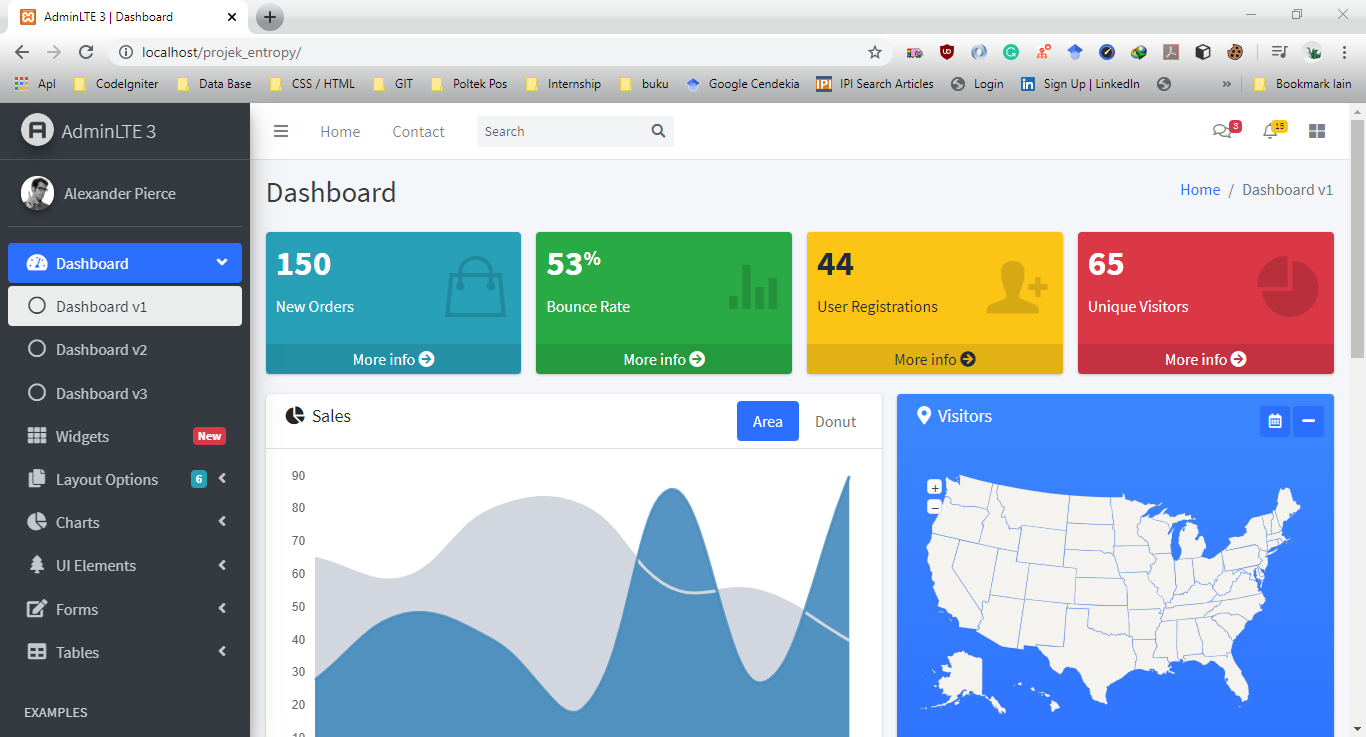
\includegraphics[width=0.90\textwidth]{figures/tmp/4.png}}
	\caption{Tampilan Awal Template Admin LTE}
	\label{tmp5}
\end{figure}

untuk fitur yang terdapat pada template pada gambar \ref{tmp5} tersebut tidak diambil semuanya melainkan di ambil sesuai dengan kebutuhan dari penggunaan sistem yang sedang dan atau akan dibangun.

\subsection{Implementasi Program}

Setelah membuat database, setting konfigurasi codeigniter kemudian penerapan template pada codeigniter, dilanjutkan dengan implementasi program, dimana perogram ini disisipkan metode atau algoritma entropy pada bagian sub modulnya, akan tetapi dikarenakan data untuk dilakukannya metode entropy harus di olah terlebi dahulu maka pada program ini dilengkapi dengan:
\begin{itemize}
\item Fitu CRUD (ceate, read, update, dan delete)
\item Fitur template yang telah di bahas pada sub bab sebelumnya 
\item Fitur login session multi user
\item Terdiri dari dua user (user admin dan user pengambil keputusan)
\item Fitur entropy
\item Terdapat enkripsi data untuk password
\end{itemize}

Dalam implementasi Program ini perlu di buat file-file dan folder terlebihdahulu pada subdirektori codeigniter yang terdapat pada controller, model, view, serta library. 

Pada gambar \ref{dir1} berikut merupakan file PHP yang dibuat pada sub direktori Controllers

\begin{figure}[!htbp]
	\centerline{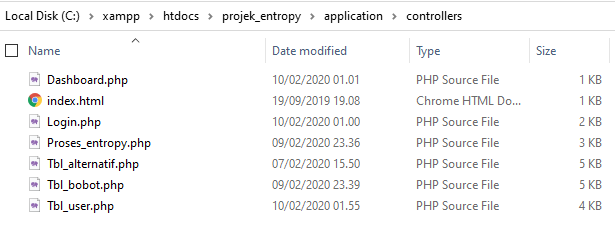
\includegraphics[width=0.90\textwidth]{figures/dir/1.png}}
	\caption{File-File Yang terdapat pada direktori Controllers}
	\label{dir1}
\end{figure}
\pagebreak
Kemudian setelah membuat file PHP pada direktori aplication/controllers  buat file PHP pada sub direktori applications/models dengan nama file seperti pada gambar \ref{dir2} berikut

\begin{figure}[!htbp]
	\centerline{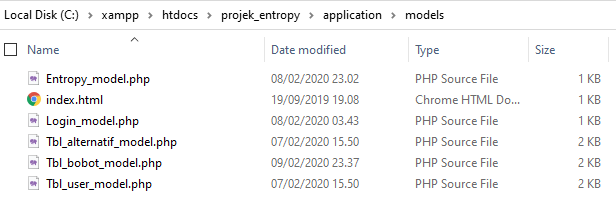
\includegraphics[width=0.90\textwidth]{figures/dir/2.png}}
	\caption{File-File Yang terdapat pada direktori Models}
	\label{dir2}
\end{figure}

Kemudian setelah membuat file PHP pada direktori applications/models buat file PHP pada sub direktori applications/libraries dengan nama file seperti pada gambar \ref{dir3} berikut

\begin{figure}[!htbp]
	\centerline{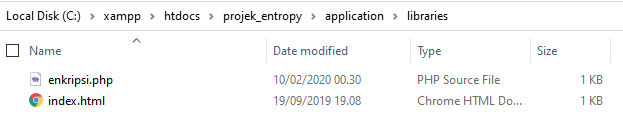
\includegraphics[width=0.90\textwidth]{figures/dir/3.png}}
	\caption{File Yang terdapat pada direktori Models}
	\label{dir3}
\end{figure}
Kemudian setelah itu pada sub direktori view buat terlebi dahulu 5 folder untuk memisahkan view dari setiap controller selain itu penempatan file juga akan menjadi lebih tertata. Adapun 5 folder itu yaitu:
\begin{itemize}
\item	Folder layout
\item	Folder entropy 
\item	Folder tbl\_alternatif
\item	Folder tbl\_bobot
\item	Folder tbl\_user 
\end{itemize}
\pagebreak 
Selain kelima folder tersebut pada subdirektori views buat dua file PHP yaitu file dashboard.php dan login.php
Untuk lebihjelasnya dapat dilihat pada gambar \ref{dir4}  berikut:

\begin{figure}[!htbp]
	\centerline{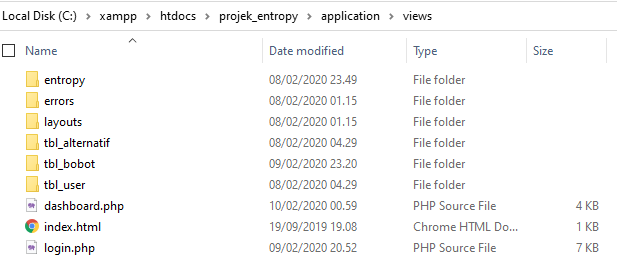
\includegraphics[width=0.90\textwidth]{figures/dir/4.png}}
	\caption{Folder dan File Yang terdapat pada direktori Views}
	\label{dir4}
\end{figure}

Untuk folder errors dan file index.html merupakan bawaan dari codeigniter, kemudian setelah kelima folder tersebut telah dibuat didalam folder tersebut buat file PHP.\\

Dimana Ketentuan untuk isi folder entropy terdiri dari dua file php yang terdiri dari hasil.php dan index.php\\
untuk lebih jelasnya seperti pada gambar \ref{dir5} berikut ini:

\begin{figure}[!htbp]
	\centerline{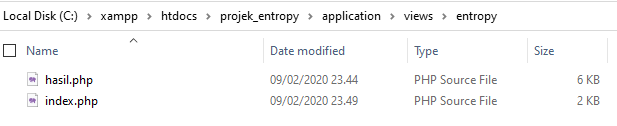
\includegraphics[width=0.90\textwidth]{figures/dir/5.png}}
	\caption{File Yang terdapat pada folder Entropy}
	\label{dir5}
\end{figure}

Kemudian untuk folder layouts buat satu file php yaitu main.php
Jelasnya seperti gambar \ref{dir6} berikut


\begin{figure}[!htbp]
	\centerline{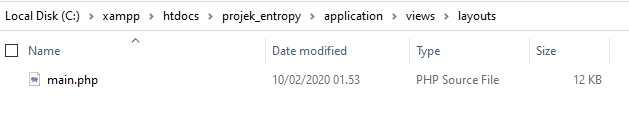
\includegraphics[width=0.90\textwidth]{figures/dir/6.png}}
	\caption{File Yang terdapat pada folder layouts}
	\label{dir6}
\end{figure}

Untuk folder tbl\_alternatif buat tiga file php terdiri dari add.php , edit.php dan index.php, jelasnya seperti pada gambar \ref{dir7} berikut:

\begin{figure}[!htbp]
	\centerline{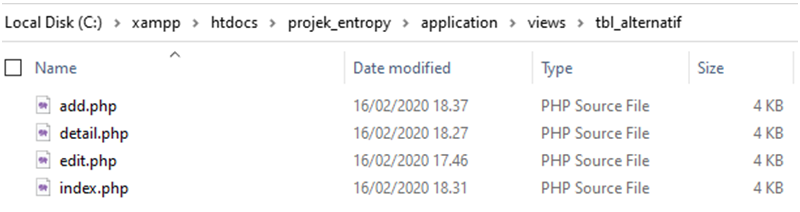
\includegraphics[width=0.90\textwidth]{figures/dir/7.png}}
	\caption{File Yang terdapat pada folder tbl\_alternatif}
	\label{dir7}
\end{figure}

Untuk folder tbl\_bobot buat tiga file php terdiri dari add.php , edit.php dan index.php, jelasnya seperti pada gambar \ref{dir8} berikut:

\begin{figure}[!htbp]
	\centerline{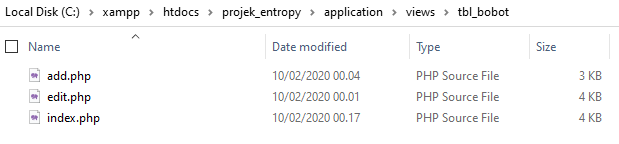
\includegraphics[width=0.90\textwidth]{figures/dir/8.png}}
	\caption{File Yang terdapat pada folder tbl\_bobot}
	\label{dir8}
\end{figure}

Untuk folder tbl\_user buat tiga file php terdiri dari add.php , edit.php dan index.php, jelasnya seperti pada gambar \ref{dir9} berikut:

\begin{figure}[!htbp]
	\centerline{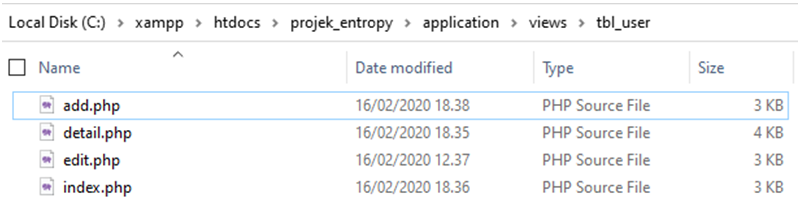
\includegraphics[width=0.90\textwidth]{figures/dir/9.png}}
	\caption{File Yang terdapat pada folder tbl\_user}
	\label{dir9}
\end{figure}

\textbf{Catatan :}\par
\textit{Untuk semua file yang telah di buat baik pada controller, model, library, maupun pada view kosongkan terlebih dahulu, hal ini untuk menghindari adanya error saat melakukan pembuatan kode}\par



\pagebreak
Tahap selanjutnya yaitu memulai coding untuk tampilan dashboard, buka file Dashboard.php yang terdapat pada file controller kemudian tuliskan source code berikut: 



\begin{lstlisting}[language=PHP]
	<?php  
	defined('BASEPATH') or exit('No direct script access allowed');  
	
	class Dashboard extends CI_Controller  
	{  
	    public function index()  
	    {  
	        if ($this->session->userdata('user_level') === 'admin') {  
	            $data['_view'] = 'dashboard';  
	            $this->load->view('layouts/main', $data);  
	        } elseif ($this->session->userdata('user_level') === 'user') {  
	            $data['_view'] = 'dashboard';  
	            $this->load->view('layouts/main', $data);  
	        } else {  
	            echo "Access Denied";  
	            redirect('login/index');  
	        }  
	    }  
	}  
\end{lstlisting}

Adapun penjelasan dari source code tersebut seperti berikut:
Dikarenakan file ini berekstensi PHP sehingga source code tersebut di buka dengan tag php kemudian di buat class yang penamaannya harys sama seperti nama file kemudian class tersebut dikarenakan berada pada controller sehingga ekstends kepada class CI\_Controller yang merupakan class bawaan dari Framework CodeIgniter.\par
Lalu pada class tersebut terdapat fungsi atau method index, method indeks merupakan fungsi yang paling pertama di jalankan (running) jika class controller tersebut dipanggil pada url. Sedangkan pada method index tersebut berisikan sour code if dan else dengan ketentuan jika data session untuk user level isinya sama dengan admin maka akan memunculkan tampilan untuk admin, kemudian jika session untuk user level isinya sama dengan user maka tampilan yang akan muncul merukana tampilan untuk user kemudian jika kedua statement berikut tidak tepenugi maka akan muncul ke halaman login. Atau masuk ke halaman yang tidak ada tampilannya.\par

Source code tersebut menjalankan view untuk halaman utama dari sistem, untuk selanjutnya buka file main.php yang terdapat pada folder view terdapat pada folder layouts kemudian isikan source code tersebut.\par
Source code tersebut berda tag HTML sehingga terbagi menjadi bagian head dan body brikut merupakan source code untuk bagian head\par
\pagebreak
\begin{lstlisting}[language=PHP]
	<!DOCTYPE html>  
	<html>  
	  
	<head>  
	    <meta charset="utf-8">  
	    <meta http-equiv="X-UA-Compatible" content="IE=edge">  
	    <title>AdminLTE 3 | Dashboard</title>  
	    <!-- Tell the browser to be responsive to screen width -->  
	    <meta name="viewport" content="width=device-width, initial-scale=1">  
	    <!-- Font Awesome -->  
	    <link rel="stylesheet" href="<?php echo site_url('resources/plugins/fontawesome-free/css/all.min.css'); ?>">  
	    <!-- Ionicons -->  
	    <link rel="stylesheet" href="https://code.ionicframework.com/ionicons/2.0.1/css/ionicons.min.css">  
	    <!-- Tempusdominus Bbootstrap 4 -->  
	    <link rel="stylesheet" href="<?php echo site_url('resources/plugins/tempusdominus-bootstrap-4/css/tempusdominus-bootstrap-4.min.css'); ?>">  
	    <!-- iCheck -->  
	    <link rel="stylesheet" href="<?php echo site_url('resources/plugins/icheck-bootstrap/icheck-bootstrap.min.css'); ?>">  
	    <!-- JQVMap -->  
	    <link rel="stylesheet" href="<?php echo site_url('resources/plugins/jqvmap/jqvmap.min.css'); ?>">  
	    <!-- Theme style -->  
	    <link rel="stylesheet" href="<?php echo site_url('resources/css/adminlte.min.css'); ?>">  
	    <!-- overlayScrollbars -->  
	    <link rel="stylesheet" href="<?php echo site_url('resources/plugins/overlayScrollbars/css/OverlayScrollbars.min.css'); ?>">  
	    <!-- Daterange picker -->  
	    <link rel="stylesheet" href="<?php echo site_url('resources/plugins/daterangepicker/daterangepicker.css'); ?>">  
	    <!-- summernote -->  
	    <link rel="stylesheet" href="<?php echo site_url('resources/plugins/summernote/summernote-bs4.css'); ?>">  
	    <link rel="stylesheet" href="<?php echo site_url('resources/plugins/datatables-bs4/css/dataTables.bootstrap4.css'); ?>">  
	    <!-- Google Font: Source Sans Pro -->  
	    <link href="https://fonts.googleapis.com/css?family=Source+Sans+Pro:300,400,400i,700" rel="stylesheet">  
	</head>
\end{lstlisting}

Pada source code head tersebut sama seperti source code untuk template, pada source code header tersebut terdapat tag title yang di gunakan untuk judul website biasanya hasilnya muncul pada tab web browser, selain tag tersebut pada header ini terdapat link-link yang menghubungkan library css yang di gunakan pada website ini library tersebut bisa onlone maupun offline, untuk memperjelas berikut merupakan contoh link yang di gunakan secara online \par

\begin{lstlisting}[language=PHP]
<link href="https://fonts.googleapis.com/css?family=Source+Sans+Pro:300,400,400i,700" rel="stylesheet">
\end{lstlisting}

\pagebreak
Sedangkan untuk link library yang digunakan secara offline seperti berikut:
\begin{lstlisting}[language=PHP]
<link rel="stylesheet" href="<?php echo site_url('resources/css/adminlte.min.css'); ?>">
\end{lstlisting}

Yang dimaksud link secara offline dikarenakan library dari css tersedia pada direktory codeignter sendiri yang di pindahkan dari direktory tempalte yang telah di unduh, kemudian utuk menjalankan link tersebur menggunakan library url, ini yang menjadikan sebab pada file autoload untuk library helper harus menambahkan url, lalu untuk arti dari link tersebut berari link tersebut mengakses folder resources kemudian mengakses folder css kemudian mengakses file adminlte.min.css, dengan catatan semua folder dan file tersebut harus berada pada folder yang digunakan untuk projek atau pada direktori codeigniter yang di jadikan projek\par
	Setelah source code pada bagian header selesai dilanjutkan dengan source code untuk bagian body, untuk souce code pada bagian body ini akan di bagi bagi meliputi penjelasan tentang navbar, sidebar, isi atau konten, kemudian footer, maka dari itu berikut merupakan source code body untuk navbar:\par


\begin{lstlisting}[language=PHP]
	<body class="hold-transition sidebar-mini layout-fixed">  
	    <div class="wrapper">  
	  
	        <!-- Navbar -->  
	        <nav class="main-header navbar navbar-expand navbar-white navbar-light">  
	            <!-- Left navbar links -->  
	            <ul class="navbar-nav">  
	                <li class="nav-item">  
	                    <a class="nav-link" data-widget="pushmenu" href="#"><i class="fas fa-bars"></i></a>  
	                </li>  
	            </ul>  
	            <!-- Right navbar links -->  
	            <ul class="navbar-nav ml-auto">  
	                <li class="nav-item">  
	                    <a class="nav-link" data-widget="control-sidebar" data-slide="true" href="#">  
	                        <i class="fas fa-th-large"></i>  
	                    </a>  
	                </li>  
	            </ul>  
	        </nav
\end{lstlisting}

Source code tersebut merupakan kelanjutan dari source kode head, pada source code tersebut di buka dengan tag body yang di sertai dengan nama class, dimana clas tersebut merupakan class yang di ambil dari file css adminlte. Kemudian pada baris 5 merupakan tag pembuka dari navbar. Kemudian dilanjutkan membuat item pada navbar pada navbar tersebut di buat dua item yang pertama di gunakan untuk menggulung sidebar kemudian item yang kedua di gunakan untuk merubah tampilan navbar dan sidebar. Untuk navar itu sendir merupakan navigator bar yang biasanya berada pada bagian atas website biasanya berisi item-item menu yang di gunakan untuk membuka halaman lain atau lain sebagainya untuk tampilan navbar sederhana seperti pada gambar \ref{ve1} berikut:\par


\begin{figure}[!htbp]
	\centerline{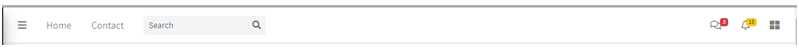
\includegraphics[width=0.90\textwidth]{figures/view/1.png}}
	\caption{contoh nav bar sederhana}
	\label{ve1}
\end{figure}


setelah navbar di buat dilanjutkan dengan membuat sidebar, sidebar itu sendiri merupakan navbar yang berada pada di pinggir untuk tampilan website bisa berada pada bagian kiri website atau pada bagian kanan website.\par
Berikut merupakan source code untuk sidebar

\begin{lstlisting}[language=PHP]
	        <aside class="main-sidebar sidebar-dark-primary elevation-4">  
	            <!-- Brand Logo -->  
	            <a href="index3.html" class="brand-link">  
	                <img src="<?php echo site_url('resources/img/APK.png'); ?>" alt="AdminLTE Logo" class="brand-image img-circle elevation-3" style="opacity: .8">  
	                <span class="brand-text font-weight-light">Aplikasi Entropy</span>  
	            </a>  
	  
	            <!-- Sidebar -->  
	            <div class="sidebar">  
	                <!-- Sidebar user panel (optional) -->  
	                <div class="user-panel mt-3 pb-3 mb-3 d-flex">  
	                    <div class="image">  
	                        <img src="<?php echo site_url('resources/img/USER.png'); ?>" class="img-circle elevation-2" alt="User Image">  
	                    </div>  
	                    <div class="info">  
	                        <a href="#" class="d-block"><?= $this->session->userdata('user_name'); ?></a>  
	                    </div>  
	                </div>  
	                <?php if ($this->session->userdata('user_level') === 'admin') { ?>  
	                    <nav class="mt-2">  
	                        <ul class="nav nav-pills nav-sidebar flex-column" data-widget="treeview" role="menu" data-accordion="false">  
	  
	                            <a href="<?= site_url('dashboard/index'); ?>" class="nav-link active">  
	                                <i class="nav-icon fas fa-tachometer-alt"></i>  
	                                <p>  
	                                    Dashboard  
	                                </p>  
	                            </a>  
	  
	                            <li class="nav-item">  
	                                <a href="<?php echo site_url('tbl_user'); ?>" class="nav-link">  
	                                    <i class="nav-icon fas fa-user-circle"></i>  
	                                    <p>  
	                                        Data User  
	                                    </p>  
	                                </a>  
	                            </li>  
	                            <li class="nav-item has-treeview">  
	                                <a href="<?php echo site_url('tbl_alternatif'); ?>" class="nav-link">  
	                                    <i class="nav-icon fas fa-file-alt"></i>  
	                                    <p>  
	                                        Data Alternatif  
	                                    </p>  
	                                </a>  
	                            </li>  
	                            <li class="nav-item has-treeview">  
	                                <a href="<?php echo site_url('proses_entropy'); ?>" class="nav-link">  
	                                    <i class="nav-icon fas fa-edit"></i>  
	                                    <p>  
	                                        Proses Entropy  
	                                    </p>  
	                                </a>  
	                            </li>  
	                            <li class="nav-item has-treeview">  
	                                <a href="<?php echo site_url('login/logout'); ?>" class="nav-link">  
	                                    <i class="nav-icon fas fa-sign-out-alt"></i>  
	                                    <p>  
	                                        Sign Out  
	                                    </p>  
	                                </a>  
	                            </li>  
	                        </ul>  
	                    </nav>  
	                <?php } elseif ($this->session->userdata('user_level') === 'user') { ?>  
	                    <nav class="mt-2">  
	                        <ul class="nav nav-pills nav-sidebar flex-column" data-widget="treeview" role="menu" data-accordion="false">  
  
	                            <a href="<?= site_url('dashboard/index'); ?>" class="nav-link active">  
	                                <i class="nav-icon fas fa-tachometer-alt"></i>  
	                                <p>  
	                                    Dashboard  
	                                </p>  
	                            </a>  
	                            <li class="nav-item has-treeview">  
	                                <a href="<?php echo site_url('tbl_alternatif/index_user'); ?>" class="nav-link">  
	                                    <i class="nav-icon fas fa-file-alt"></i>  
	                                    <p>  
	                                        Data Alternatif  
	                                    </p>  
	                                </a>  
	                            </li>  
	                            <li class="nav-item has-treeview">  
	                                <a href="<?php echo site_url('proses_entropy/proses_user'); ?>" class="nav-link">  
	                                    <i class="nav-icon fas fa-edit"></i>  
	                                    <p>  
	                                        Proses Entropy  
	                                    </p>  
	                                </a>  
	                            </li>  
	                            <li class="nav-item has-treeview">  
	                                <a href="<?php echo site_url('login/logout'); ?>" class="nav-link">  
	                                    <i class="nav-icon fas fa-sign-out-alt"></i>  
	                                    <p>  
	                                        Sign Out  
	                                    </p>  
	                                </a>  
	                            </li>  
	                        </ul>  
	                    </nav>  
	                <?php } ?>  
	                <!-- Sidebar Menu -->  
	  
	                <!-- /.sidebar-menu -->  
	            </div>  
	            <!-- /.sidebar -->  
	        </aside>
\end{lstlisting}


Source code tersebut merupakan source code kelanjutan dari source code navbar, pada source code tersebut menggunakan clausa if dan elseif yang terdapat pada baris ke 19 dan baris ke 64  dengan parameter session hal ini di lakukan untuk menampilkan sidebar yang berbeda untuk setiap user level. Kemudian untuk contoh side bar yang di gunakan pada sistem ini untuk user level samadengan admin maka seperti pada gambar \ref{ve3} kemudian untuk user level samadengan user maka sidebarnya seperti gambar \ref{ve2} berikut ini:
\pagebreak
\begin{figure}[!htbp]
	\centerline{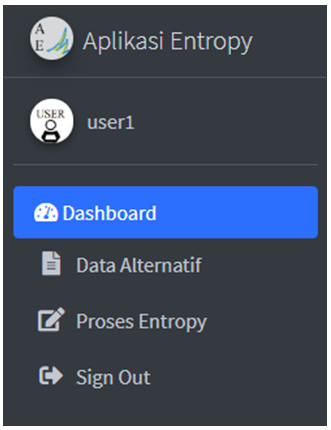
\includegraphics[width=0.50\textwidth]{figures/view/2.png}}
	\caption{Side Bar Untuk User}
	\label{ve2}
\end{figure}

\begin{figure}[!htbp]
	\centerline{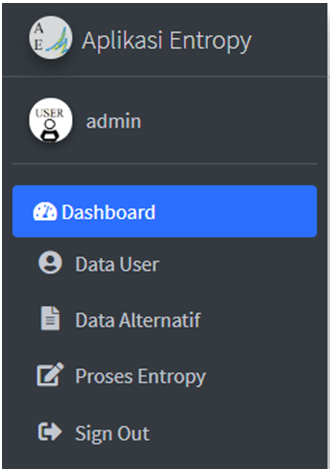
\includegraphics[width=0.50\textwidth]{figures/view/3.png}}
	\caption{Side Bar Untuk User}
	\label{ve3}
\end{figure}

setelah itu dilanjutkan dengan menambahkan \textit{source code content} yang merupakan tampilan atau  isi dari laman website tersebut,  berikut merupakan \textit{source code} dari content: 

\begin{lstlisting}[language=PHP]
	        <div class="content-wrapper">  
	            <!-- Content Header (Page header) -->  
	            <?php  
	            if (isset($_view) && $_view)  
	                $this->load->view($_view);  
	            ?>  
	            <!-- /.content -->  
	        </div>
\end{lstlisting}
\textit{Pada source code} tersebut di gunakan untuk menarik \textit{content} untuk tampilan tersebut sesuai pada nilai pada variabel \$\_view pada variabel tersebut berisikan data berupa string yaitu  nama tampilan yang akan di load atau di peroses, nama tampilan tersebut dikirim dari \textit{controller} yang berkaitan dengan variabel tersebut maka dari itu source code main.php bisa di gunakan dan di kombinasikan dengan semua file yang terdapat pada view. kemudian setelah \textit{content} maka di akhiri dengan source code footer seperti berikut\par

\begin{lstlisting}[language=PHP]
	<footer class="main-footer">  
	            <strong>Copyright &copy; 2020</strong>  
	            Aplikasi Entropy.  
	            <div class="float-right d-none d-sm-inline-block">  
	                <b>Version</b> 1.0  
	            </div>  
	        </footer>  
	    </div>  
\end{lstlisting}
Source code tersebut digunakan sebagai footer dimana berisikan data copyright dari web atau informasi lain bisa berupa versi dari website atau bisa berisi email dari pemilik website, untuk contoh dari footer seperti pada gambar berikut:\par

\begin{figure}[!htbp]
	\centerline{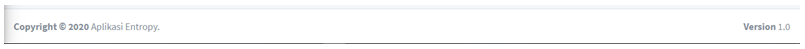
\includegraphics[width=0.90\textwidth]{figures/view/4.png}}
	\caption{Contoh Footer}
	\label{ve4}
\end{figure}

lalu perbedaan antara footer yang di bahas tadi dengan footer yang sekarang yaitu pada footer yang di gunakan pada template merupakan footer yang di gunakan untuk memanggil library java script sedangkan footer pada gambar \ref{ve4} merupakan footer yang digunakan untuk content atau untuk tampilan website.\par
\pagebreak
Setelah itu dilanjutkan dengan dengan source code untuk memanggil library dari javascript yang di gunakan pada sistem atau yang sering di sebut footer juga, untuk detail source codenya seperti berikut:

\begin{lstlisting}[language=PHP]
	    <!-- jQuery -->  
	    <script src="<?php echo site_url('resources/plugins/jquery/jquery.min.js'); ?>"></script>  
	    <!-- jQuery UI 1.11.4 -->  
	    <script src="<?php echo site_url('resources/plugins/jquery-ui/jquery-ui.min.js'); ?>"></script>  
	    <!-- Resolve conflict in jQuery UI tooltip with Bootstrap tooltip -->  
	    <script>  
	        $.widget.bridge('uibutton', $.ui.button)  
	    </script>  
	    <!-- Bootstrap 4 -->  
	    <script src="<?php echo site_url('resources/plugins/bootstrap/js/bootstrap.bundle.min.js'); ?>"></script> 
	    <!-- ChartJS -->  
	    <script src="<?php echo site_url('resources/plugins/chart.js/Chart.min.js'); ?>"></script>  
	    <!-- Sparkline -->  
	    <script src="<?php echo site_url('resources/plugins/sparklines/sparkline.js'); ?>"></script>  
	    <!-- JQVMap -->  
	    <script src="<?php echo site_url('resources/plugins/jqvmap/jquery.vmap.min.js'); ?>"></script>  
	    <script src="<?php echo site_url('resources/plugins/jqvmap/maps/jquery.vmap.usa.js'); ?>"></script>  
	    <!-- jQuery Knob Chart -->  
	    <script src="<?php echo site_url('resources/plugins/jquery-knob/jquery.knob.min.js'); ?>"></script>  
	    <!-- daterangepicker -->  
	    <script src="<?php echo site_url('resources/plugins/moment/moment.min.js'); ?>"></script>  
	    <script src="<?php echo site_url('resources/plugins/daterangepicker/daterangepicker.js'); ?>"></script>  
	    <!-- Tempusdominus Bootstrap 4 -->  
	    <script src="<?php echo site_url('resources/plugins/tempusdominus-bootstrap-4/js/tempusdominus-bootstrap-4.min.js'); ?>"></script>  
	    <!-- Summernote -->  
	    <script src="<?php echo site_url('resources/plugins/summernote/summernote-bs4.min.js'); ?>"></script>  
	    <!-- overlayScrollbars -->  
	    <script src="<?php echo site_url('resources/plugins/overlayScrollbars/js/jquery.overlayScrollbars.min.js'); ?>"></script>  
	    <!-- AdminLTE App -->  
	    <script src="<?php echo site_url('resources/js/adminlte.js'); ?>"></script>  
	    <!-- AdminLTE dashboard demo (This is only for demo purposes) -->  
	    <script src="<?php echo site_url('resources/js/pages/dashboard.js'); ?>"></script>  
	    <!-- AdminLTE for demo purposes -->  
	    <script src="<?php echo site_url('resources/js/demo.js'); ?>"></script>  
	    <script src="<?php echo site_url('resources/plugins/datatables/jquery.dataTables.js'); ?>"></script>  
	    <script src="<?php echo site_url('resources/plugins/datatables-bs4/js/dataTables.bootstrap4.js'); ?>"></script>  
	    <script>  
	        $(function() {  
	            $("#example1").DataTable();  
	            $('#example2').DataTable({  
	                "paging": true,  
	                "lengthChange": false,  
	                "searching": false,  
	                "ordering": true,  
	                "info": true,  
	                "autoWidth": false,  
	            });  
	        });  
	    </script>
	</body>
	</html>
\end{lstlisting}

	Pada dasarnya soucode tersebut sama seperti sour code header, pada source code tersebut memanggil library javascript atau js yang di gunakan pada sistem ini, tidak hanya library js ada juga pengaturan utuk tabel atau data tabel menggunakan java script yang di kombinasikan dengan css pada tabel yang terdapat pada content.\par
	Untuk code keseluruhan atau lengkap code dari file main.php dan file dashboard.php pada controller dapat di lihat pada daftar source code sistem pada  source code main.php dan daftar source code sistem pada  source code dashboard.php controller\par
Adapun isi dari konten untuk dashboard terdapat pada file Dashboard.php yang terdapat pada folder view sebagai berikut,  pada file tersebut berisikan card-card yang di gunakan untuk user admin dan user\par

\begin{lstlisting}[language=PHP]
	<div class="content-header">
	    <div class="container-fluid"> 
	        <div class="row mb-2">  
	            <div class="col-sm-6">  
	                <h1 class="m-0 text-dark">Dashboard</h1>  
	            </div><!-- /.col -->  
	        </div><!-- /.row -->  
	    </div><!-- /.container-fluid -->  
	</div>  
	<!-- /.content-header -->  
	  
	<!-- Main content -->  
	<section class="content">  
	    <div class="container-fluid">  
	        <!-- Small boxes (Stat box) -->  
	        <?php if ($this->session->userdata('user_level') === 'admin') { ?>  
	            <div class="row">  
	                <div class="col-lg-4 col-6">  
	                    <!-- small box -->  
	                    <div class="small-box bg-info">  
	                        <div class="inner"> 
	                            <h3></h3>  
	  
	                            <p>Data Alternatif</p>  
	                        </div>  
	                        <div class="icon">  
	                            <i class="ion ion-document"></i>  
	                        </div>  
	                        <a href="<?= base_url('tbl_alternatif') ?>" class="small-box-footer">More info <i class="fas fa-arrow-circle-right"></i></a>  
	                    </div> 
	                </div>  
	                <!-- ./col -->  
	                <div class="col-lg-4 col-6">  
	                    <!-- small box -->  
	                    <div class="small-box bg-success">  
	                        <div class="inner">  
	                            <h3></h3>  
	  
	                            <p>Data Bobot</p>  
	                        </div>  
	                        <div class="icon">  
	                            <i class="ion ion-stats-bars"></i>  
	                        </div>  
	                        <a href="<?= base_url('tbl_bobot') ?>" class="small-box-footer">More info <i class="fas fa-arrow-circle-right"></i></a>  
	                    </div>  
	                </div>  
	                <!-- ./col -->  
	                <div class="col-lg-4 col-6">  
	                    <!-- small box -->  
	                    <div class="small-box bg-warning">  
	                        <div class="inner">  
	                            <h3></h3>  
	  
	                            <p>Data User</p>  
	                        </div>  
	                        <div class="icon">  
	                            <i class="ion ion-person-add"></i>  
	                        </div>  
	                        <a href="<?= base_url('tbl_user'); ?>" class="small-box-footer">More info <i class="fas fa-arrow-circle-right"></i></a> 
	                    </div>  
	                </div>  
	                <!-- ./col -->  
	            </div>  
	        <?php } elseif ($this->session->userdata('user_level') === 'user') { ?>  
	            <div class="row">  
	                <div class="col-lg-6 col-6">  
	                    <!-- small box -->  
	                    <div class="small-box bg-info">  
	                        <div class="inner">  
	                            <h3></h3>  
	  
	                            <p>Data Alternatif</p>  
	                        </div>  
	                        <div class="icon">  
	                            <i class="ion ion-document"></i>  
	                        </div>  
	                        <a href="<?= base_url('tbl_alternatif/index_user') ?>" class="small-box-footer">More info <i class="fas fa-arrow-circle-right"></i></a>  
	                    </div>  
	                </div>  
	                <!-- ./col -->  
	                <div class="col-lg-6 col-6">  
	                    <!-- small box -->  
	                    <div class="small-box bg-success">  
	                        <div class="inner">  
	                            <h3></h3>  
	  
	                            <p>Data Bobot</p>  
	                        </div>  
	                        <div class="icon">  
	                            <i class="ion ion-stats-bars"></i>  
	                        </div>  
	                        <a href="<?= base_url('tbl_bobot') ?>" class="small-box-footer">More info <i class="fas fa-arrow-circle-right"></i></a>  
	                    </div>  
	                </div>  
	                <!-- ./col -->  
	            </div>  
	        <?php } ?>  
	    </div><!-- /.container-fluid -->  
	</section>  
\end{lstlisting}

Kemudian pada source code tersebut menggunakan kausa if dan elseif yang digunakan untuk memisahkan konten yang di tampilkan untuk setiap user levelnya, secara logika cara tersebut mirip dengan cara if dan elseif yang di gunakan untuk navbar dan yang di gunakan pada file Dashboard yang terdapat pada controller, lalu untuk lengkapnya source code tersebut dapat di lihat pada daftar source code sistem pada subbab source code dashboard pada kode file view  dashboard.php\par
Untuk tampilannya seperti pada gambar \ref{ve5} dan pada gambar \ref{ve6}
\pagebreak
\begin{figure}[!htbp]
	\centerline{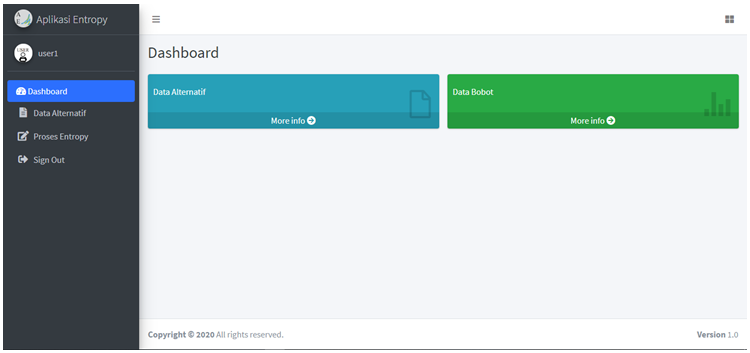
\includegraphics[width=0.90\textwidth]{figures/view/5.png}}
	\caption{view dashboard untuk user}
	\label{ve5}
\end{figure}

pada gambar \ref{ve5} merupakan tampilan dashboard untuk user, dimana pada dahboard tersebut menampilkan dua card didalamnya terdapat link untuk mengakses data alternatif dan data bobot.


\begin{figure}[!htbp]
	\centerline{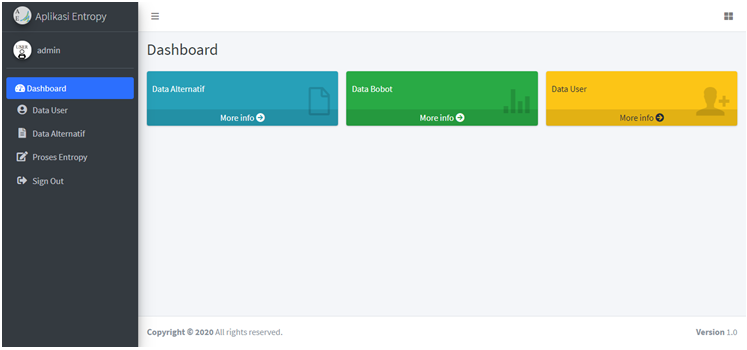
\includegraphics[width=0.90\textwidth]{figures/view/6.png}}
	\caption{view dashboard untuk admin}
	\label{ve6}
\end{figure}

pada gambar \ref{ve5} merupakan tampilan dashboard untuk user, dimana pada dahboard tersebut menampilkan tiga card didalamnya terdapat link untuk mengakses data alternatif , data bobot dan data user

Adapun syarat ke dua dashboard itu muncul yaitu dengan melakukan login pada sistem, jika telah melakukan login maka dashboard akan muncul sesuai dengan user level yang melakukan login pada sistem.\par

Oleh karena itu berikut merupakan source code login mulai dari controller, model, dan view untuk login, adapun penjelasan source code Login.php pada controller seperti berikut:\par
\pagebreak
\begin{lstlisting}[language=PHP]
	<?php  
	defined('BASEPATH') or exit('No direct script access allowed');  
	  
	class Login extends CI_Controller  
	{  
	    function __construct()  
	    {  
	        parent::__construct();  
	        $this->load->model('login_model');  
	        $this->load->library('enkripsi');  
	    } 
\end{lstlisting}

Adapun pada source code Login di buat terlebih dahulu class dengan nama Login dengan ekstensi ke class CI\_Controller, sama seperti pada file Dashboard.php di controller nama file dan class harus sama, setelah membuat class dilanjutkan pada baris ke 6 dengan membuat fungsi construktor yang berpungsi sebagi parent yang dapat di gunakan di semu fungsi yang berada pada class tersebut, pada source code tersebut di fungsi contruktor melakukan load atau memanggil model dengan nama class login\_model dan memanggil library dengan nama class enkripsi, untuk class enkripsi akan di jelaskan setelah pembahasan controller Login.php, jika source code tersebut telah di buat di lanjutkan dengan menambahkan fungsi seperti berikut:\par

\begin{lstlisting}[language=PHP]
	 public function index()  
	    {  
	        $this->form_validation->set_rules('username', 'username', 'required');  
	        $this->form_validation->set_rules('password', 'Password', 'required|min_length[4]');  
	        if ($this->form_validation->run() == FALSE) {  
	  
	            $this->load->view('login'); 
	        } else {  
	            $username    = $this->input->post('username', TRUE);  
	            $password = $this->enkripsi->encryptIt($this->input->post('password', TRUE));  
	            $validasi = $this->login_model->validate($username, $password);  
	            if ($validasi->num_rows() > 0) {  
	                $data  = $validasi->row();  
	                $id    = $data->user_id;  
	                $level = $data->user_level;  
	                $user_name = $data->user_name; 
	                $sesiondata = array(  
	                    'user_id'  => $id,  
	                    'user_level'     => $level,  
	                    'user_name' => $user_name,  
	                    'logged_in' => TRUE  
	                );  
	                $this->session->set_userdata($sesiondata);  
	  
	                if ($level === 'admin') { 
	                    redirect('dashboard');  
	                } elseif ($level === 'user') {  
	                    redirect('dashboard');  
	                }  
	            } else {  
	                echo $this->session->set_flashdata('msg', 'Username or Password is Wrong');  
	                redirect('');  
	            }  
	        }  
	    } 
\end{lstlisting}

Fungsi atau method pada souce code tersebut di gunakan sebagai logika untuk login pada sistem, adapun penjelasannya seperti berikut: fungsi tersebut menggunakan nama index yang berarti jika kelas Login di panggil berarti fungsi yang terlebih dahulu dijalankan maka fungsi tersebut, kemudian dilanjutkan dengan form\_validation pada baris ke 3 dan 4 yang di gunakan untuk validasi dari form insert data yang di gunakan untuk login, pada form\_validation tersebut memiliki aturan untuk form dengan ekstensi name username pada view wajib di isi kemudian untuk form dengan ekstensi name password pada view wajib di isi dan memiliki minimal panjang karakter yaitu 4 karakter.\par
	Selanjutnya pada baris ke 5 nilai dari form\_validation tersebut di jadikan parameter untuk if else dengan status form\_validation bernilai false atau salah hal ini bisa berarti form\_validation yang belum berisi nilai atau data yang dimasukan tidak sesuai dengan aturan form\_validation maka jika kedua syarat tersebut terpenuhi maka akan menjalankan view (tampilan) dari login, namun jika form\_validation berisi nilai maka di lanjutkan ke baris 9 dan 10 dimana terdapat dua variabel \$username yang di gunakan untuk menangkap nilai dari form username menggunakan method post begitu pula untuk variabel \$password namun pariabel tersebut dilakukan enkripsi data sehingga data yang ditangkap di ubah menjadi kode.\par
	Kemudian pada baris ke 11 dilakukan validasi yaitu dengan cara membuat variabel \$validasi yang berisikan model dan fungsinya, model dan fungsinya tersebut dimasukan nilai dari variabel \$username dan \$password kemudian pada model dilakukan perbandingan data dengan data yang terdapat pada basis data jika data tersebut tidak sesuai dengan data yang terdapat pada database maka akan kembali lagi ke view untuk login lalu jika data tersebut sama dengan data yang ada di database data tersebut digunakan untuk membandingkan data yang terdapat pada satu baris pada basis data kemudian digunakan sebagai parameter untuk mebuat session.\par
	Pada baris ke 12 sampai 16 merupakan peroses pengambilan data dari database yang di gunakan untuk membuat session, kemudian data-data tersebut di masukan kedalam setiap variabel, setiap variabel tersebut di masukan kedalan array untuk penamanna sebagai contoh pada array di baris ke 18 ‘user\_id’ merupakan nama session akan di gunakan kemudian data yang terdapat pada nama tersebut terdapat pada variabel \$id.\par
	Setelah pembuatan session telah di lakukan peroses selanjutnya yaitu membandingkan data yang terdapat pada basis data berupa userlevel yang telah di jadikan variabel \$level data tersebut di bandingkan jika didalammnya terdapat data yang sama dengan karakter tulisan ‘admin’ maka akan di pindahkan ke halaman utama admin, kemudian jika nilai pada variabel tersebut bernilai ‘user’ maka akan di pindahkan ke halaman user, kemudian jika syarat-syarat tersebut tidak terpenuhi maka akan dialaihkan kembali ke class login.\par
	Kemudian jika source code tersebut telah di buat dilanjutkan dengan membuat fungsi logout, masih pada class yangsama yaitu class login, berikut merupakan source code dari fungsi logout.
\begin{lstlisting}[language=PHP]
	function logout()  
	    {  
	        $this->session->sess_destroy();  
	        redirect('Login');  
	    }  
	}  
\end{lstlisting}

Pada fungsi atau method tersebut di gunakan untuk menghapus session dari user yang telah login sehingga jika user telah melakukan logout maka session dari user tersebut telah terhapus.\par
Untuk selanjutnya dilanjutkan dengan membahas model yang di gunakan untuk controller Login.php tersebut, adapunn file yang di gunakan yaitu Login\_model yang terdapat pada subdirektory atau folder Models lalu untuk source code dari model tersebut sebagai berikut:\par

\begin{lstlisting}[language=PHP]
	<?php  
	class Login_model extends CI_Model  
	{  
	  
	    function validate($email, $password)  
	    {  
	        $this->db->where('user_name', $email);  
	        $this->db->where('user_password', $password);  
	        $result = $this->db->get('tbl_user');  
	        return $result;  
	    }  
	}  
\end{lstlisting}
Lalu untuk class Login\_model yang terdapat pada model merupakan untuk pembuatan classnya nama class harus sama seperti nama file dengan ekstensi ke CI\_Model dikarenakan terdapat pada folder model pada CodeIgniter, kemudian di dalammnya terdapat fungsi validate yang digunakan untuk menangkap data dari dua variabel yang dikirim dari controller lalu nailai pada variabel tersebut di bandingkan dengan data yang terdapat pada basis data.\par
Pada source code yang terdapat pada Login.php di controller terdapat variabel \$validasi variabel tersebut menangkap nilai dari variabel \$username dan \$password, yang kemudian nilai pada kedua variabel tersebut di kirimkan ke model yang terdapat pada file login\_model.php kemudian di tangkap oleh fungsi validate atau kalau di tuliskan pada source code seperti brikut.
\begin{verbatim}
$this->login_model->validate($username, $password) 
\end{verbatim}
yang artinya pada class controller login dipanggil class pada model dengan nama login\_model kemudian menjalankan method yang ada di dalammya dengan nama validate yang menangkap nilai dari variabel \$username dan \$password.\par

\pagebreak
Pada source code \$password dilakukan enkripsi data menggunakan class dan fungsi yang terdapat pada library, maka dari itu berikut merupakan source code yang terdapat pada folder library dengan nama enkripsi.php\par


\begin{lstlisting}[language=PHP]
	<?php  
	class Enkripsi  
	{  
	    public function encryptIt($password)  
	    {  
	        $cryptKey  = '1212';  
	        $qEncoded      = base64_encode(mcrypt_encrypt(MCRYPT_RIJNDAEL_256, md5($cryptKey), $password, MCRYPT_MODE_CBC, md5(md5($cryptKey))));  
	        return ($qEncoded);  
	    }  
	    public function decryptIt($password)  
	    {  
	        $cryptKey  = '1212';  
	        $qDecoded      = rtrim(mcrypt_decrypt(MCRYPT_RIJNDAEL_256, md5($cryptKey), base64_decode($password), MCRYPT_MODE_CBC, md5(md5($cryptKey))), "\0");  
	        return ($qDecoded);  
	    }  
	} 
\end{lstlisting}

Pada code enkripsi tersebut terdapat dua fungsi yaitu fungsi encryptIt dan fingsi decryptIt, dimana fungsi encryptIt digunakan untuk mengenkripsi data password sehingga password yang di simpan pada database telah di enkripsi sehingga berbentuk kode kemudian untuk mengurai kode tersebut (dekripsi) menggunakan fungsi decryptIt. Kedua fungsi atau kelas ini di gunakan agar user dapat melakukan login, kemudian fungsi ini juga di gunakan untuk mengelola password dari user.\par
	Setelah code pada file Login.php, Login\_model.php, dan Enkripsi.php dibuat, buka file login yang terdapat pada view kemudian masukan code berikut yang bertujuan untuk membuat tampilan form login pada sistem ini berikut merupakan souce code untuk form pada view login.php untuk lengkapnya source code untuk tampilan login dapat di lihat pada lampiran Login pada view\par

\begin{lstlisting}[language=PHP]
	<form role="form" id="quickForm" action="" method="post">  
	       <div class="card-body">  
	           <div class="form-group">  
	               <label for="exampleInputUsername1">username</label> 
	               <input type="text" name="username" class="form-control" id="exampleInputUsername1" placeholder="Enter username">  
	           </div>  
	       <div class="form-group">  
	          <label for="exampleInputPassword1">Password</label>  
	           <input type="password" name="password" class="form-control" id="exampleInputPassword1" placeholder="Password">  
	       </div>  
	    </div>  
	<!-- /.card-body -->  
	      <div class="card-footer">  
	        <button class="btn btn-primary" value="Login" name="kirim" type="submit">Sign in  
	               <i class="nav-icon fas fa-sign-in-alt"></i>  
	         </button>  
	      </div> 
	</form>  
\end{lstlisting}

Pada source code tersebut intinya terdapat pada name yang terdapat pada form input pada name tersebut terdapat nilai yang di gunakan sebagai parameter nilai name tersebut harus sama dengan variabel yang menangkapnya menggunakan method post pada controller yang bersangkutan dengan form tersebut agar lebih jelas sebagai contoh pada controller login.php terdapat source code berikut:\par

\begin{lstlisting}[language=PHP]
$username    = $this->input->post('username', TRUE);
\end{lstlisting}

Pada source code tersebut terdapat parameter yaitu username parameter itu harus sama dengan yang terdapat pada form input, kalu pada form input parameter tersebut biasanya di sisipkan pada name seperti source code berikut:

\begin{lstlisting}[language=PHP]
<input type="text" name="username" class="form-control" id="exampleInputUsername1" placeholder="Enter username">
\end{lstlisting}

Intinya nilai parameter name harus sama dengan parameter post yang terdapat pada controller yang di gunakan untuk form tersebut. kemudian berikut merupakan sekilas tampilan form login yang di gunakan pada sistem:

\begin{figure}[!htbp]
	\centerline{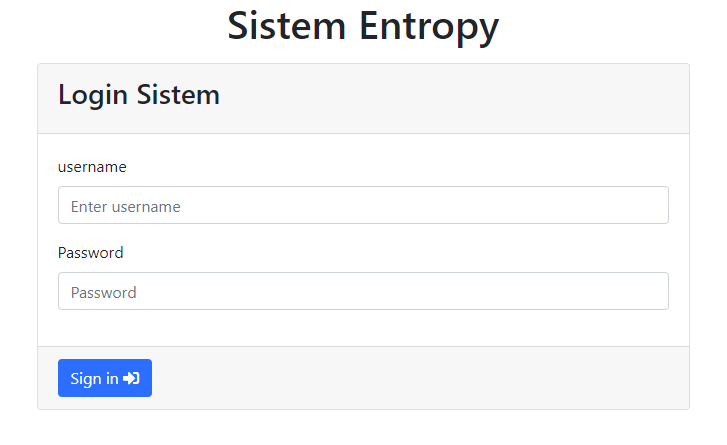
\includegraphics[width=0.90\textwidth]{figures/view/7.png}}
	\caption{Form Login Sistem}
	\label{ve7}
\end{figure}

Pada gambar \ref{ve7} tersebut merupakan form login yang terdiri dari dua inputan yaitu username dan password.

\textbf{Catatan :} 
\textit{untuk source code lengkap Login terdapat pada daftar source code sistem pada subbab source code login}\par


\pagebreak
Setelah membuat menu login dan dashboard untuk ke dua userl level dilanjutkan ke peroses CRUD data alternatif, kenapa harus CRUD data alternatif ?. itu karena data yang akan di bobotkan merupakan data kriteria yang terdapat pada data alternatif sehingga data alternatif yang dahulu diolah atau di siapkan. Maka dari itu untuk menyiapkan data alternatif perlu proses crud untuk data alternatif untuk melakukan peroses crud tentunya di butuhkan controller, model, dan view berikut merupakna code controller untuk file Tbl\_alternatif.php 

\begin{lstlisting}[language=PHP]
	<?php  
	class Tbl_alternatif extends CI_Controller  
	{  
	    function __construct()  
	    {  
	        parent::__construct();  
	        $this->load->model('Tbl_alternatif_model');  
	    }  
\end{lstlisting}

Pada file controller Tbl\_alternatif terdapat fungsi \_\_construct yang merupakan construktor dari class tersebut, kemudian pada fungsi tersebut terdapat parent::\_\_construct(); yangmerupakan induk dari code yang terdapat pada class tersebut maksud parren di sini jika ada model, helper atau library dan lain sebagainya di dekralasikan pada fungsi tersebut berarti fungsi atau class yang telah di dekralasikan tersebut dapat di gunakan pada fungsi lainnya yang terdapat pada class tersebut.
	Lalu setelah fungsi konstruktor dibuat dilanjutkan dengan membuat fungsi index yang di gunakan untuk user admin berikut merupakan source code-nya:\par
\begin{lstlisting}[language=PHP]
	function index()  
	{  
	    $data['tbl_alternatif'] = $this->Tbl_alternatif_model->get_all_tbl_alternatif_admin();  
	    $data['_view'] = 'tbl_alternatif/index';  
	    $this->load->view('layouts/main', $data);  
	}  
\end{lstlisting}

Pada fungsi tersebut digunakan untuk mengambil semua data alternatif tanpa dilakukan penyortiran, sehingga data yang muncul merupakan data yang terdapat pada tabel alternatif, selanjutnya buat fungsi index\_user, untuk source codenya seperti berikut:

\begin{lstlisting}[language=PHP]
	function index_user()  
	{ 
	    $session = $this->session->userdata('user_id'); 
	    $data['tbl_alternatif'] = $this->Tbl_alternatif_model->get_all_tbl_alternatif($session);  
	    $data['_view'] = 'tbl_alternatif/index';  
	    $this->load->view('layouts/main', $data);  
	}  
\end{lstlisting}


Pada fungsi tersebut di gunkan untuk menampilkan data alternatif berdasarkan user id dari user, sehingga untuk user yang login akan memunculkan data alternatif sesuai user yang bersangkutan kecuali pada user admin, untuk parameter yang di gunakan merupakan session dari user id dari user yang melakukan login, kemudian selanjutnya buat fungsi add untuk penjelassnyannya akan di bagi- bagi seperti berikut:\par

\begin{lstlisting}[language=PHP]
	function add()  
	    {  
	        $this->load->library('form_validation');  
	  
	        $this->form_validation->set_rules('alternatif_nama', 'Alternatif Nama', 'required|max_length[30]');  
	        $this->form_validation->set_rules('kriteria_1', 'Kriteria 1', 'required|integer');  
	        $this->form_validation->set_rules('kriteria_2', 'Kriteria 2', 'required|integer');  
	        $this->form_validation->set_rules('kriteria_3', 'Kriteria 3', 'required|integer');  
	        $this->form_validation->set_rules('kriteria_4', 'Kriteria 4', 'required|integer');  
	        $this->form_validation->set_rules('id_user', 'Id User', 'required|integer');  
	  
\end{lstlisting}


Pada bagian pertama di dalam fungsi add di jalankan form validation yang merupakan library bawaan dari codeigniter, form validation itu sendiri di gunakan sebagai validasi dari dari form yang di gunakan pada sistem, di dalamnya tersiri dari name dari form dilanjutkan dengan karekter yang akan di tampilkan sebagai notifikasi dari form validation kemmudian diakhiri dengan aturan dari form misalkan tertulis seperti berikut required|integer yang berarti form tersebut wajib di isi dengan tipe data integer (int), setelah membuat form validation di lanjutkan dengan membuat ststement if dan perogeam yang akan di jalankan jika ststement perikut terjalankan.\par

\begin{lstlisting}[language=PHP]
	        if ($this->form_validation->run()) {  
	            $params = array(  
	                'alternatif_nama' => $this->input->post('alternatif_nama'),  
	                'kriteria_1' => $this->input->post('kriteria_1'),  
	                'kriteria_2' => $this->input->post('kriteria_2'),  
	                'kriteria_3' => $this->input->post('kriteria_3'),  
	                'kriteria_4' => $this->input->post('kriteria_4'),  
	                'id_user' => $this->input->post('id_user'),  
	            );  
	  
	            $tbl_alternatif_id = $this->Tbl_alternatif_model->add_tbl_alternatif($params);  

\end{lstlisting}

Pada source code tersebut menggunakan aturan if dangan parameter dari form validation, dimana jika form validation berjalan maka akan menjalankan source code yang terdapat pada aturan if tersebut, adapun source code yang terdapat pada aturan if tersebut merupakan array yang di tampung dalam satu variabel bernama params, kemudian untuk isi array merupakan data yang di kirim dari form dengan parameter name pada form (nama masing masing form), kemudian data yang di tampung pada form tersebut di kirim ke model dengan nama Tbl\_alternatif\_model dengan nama fungsi add\_tbl\_alternatif jika semua syarat terseut maka akan menjalankan source code dengan aturan if seperti berikut:\par

\begin{lstlisting}[language=PHP]
	if ($this->session->userdata('user_level') === 'admin') {  
	                redirect('tbl_alternatif/index');  
	            } else {  
	                redirect('tbl_alternatif/index_user');  
	            }  
	        } else {  
	            $data['_view'] = 'tbl_alternatif/add';  
	            $this->load->view('layouts/main', $data);  
	        }  
	    }  
\end{lstlisting}

Source code if else tersebut digunakan memindahkan tampilan tergantung user level yang login, hal ini ditandai dengan session userlevel yang di gunakan parameter, kemudian untuk else yang kedua pada baris ke 6 merupakan sambungan dari if yang bertama, yang jika parameter form validation tidak berjalan maka akan muncul form tambah data\par
	Setelah fungsi add tambahkan fungsi edit yang di gunakan untuk mengedit atau mengkoreksi data pada dasarnya fungsi edit dan fungsi add itu sama hanya saja beda dalam menampilkan form input data tidak hanya itu perbedaanya juga terdapat pada awal fungsi yang menmeriksa apakah tabel yang akan di edit terdapat pada database dan juga pada model yang di gunakan  berikut merupakan perbedaan source codenya \par

\begin{lstlisting}[language=PHP]
	function edit($alternatif_id)  
	    {  
	        // check if the tbl_alternatif exists before trying to edit it  
	        $data['tbl_alternatif'] = $this->Tbl_alternatif_model->get_tbl_alternatif($alternatif_id);  
	  
	        if (isset($data['tbl_alternatif']['alternatif_id'])) {  
\end{lstlisting}

Pada source code fungsi edit tersebut terdapat variabel \$alternatif\_id yang digunakan untuk menangkap id yang di kitim dari tombol edit, kemudian ada klausa atau aturan if dimana aturan tersebut digunakan untuk memeriksa apakah variabel \$data dengan parameter tbl\_alternatif dan id dari tabel alternatif tersebut data nya ada atau tidak pada tabel tersebut jika data tersebut ada maka selanjutnya sama seperti proses tambah data, kemudian untuk modelnya yang berbeda seperti berikut:

\begin{lstlisting}[language=PHP]
 $this->Tbl_alternatif_model->update_tbl_alternatif($alternatif_id, $params);  
\end{lstlisting}

Pada soucode tersebut terdapat dua parameter berupa variabel yang dikirm ke model terdiri dari id dari tabel kemudian data yang di update atau di edit.\par
Kemudian setelah fungsi edit di buat dilanjutkan dengan fungsi detail yang digunakan untuk memuncul detail dari data yang di pilih, berikut merupakan source code dari data yang digunakan untuk melakukan detail data:\par

\begin{lstlisting}[language=PHP]
	    function detail($alternatif_id)  
	    {  
	        $data['tbl_alternatif'] = $this->Tbl_alternatif_model->get_tbl_alternatif($alternatif_id);  
	        $data['_view'] = 'tbl_alternatif/detail';  
	        $this->load->view('layouts/main', $data);  
	    }
\end{lstlisting}

Pada source code tersebut menggunakan parameter id yang dikirim melalui tombol hampirsama seperti peroses edit, kemudian untuk model yang di gunakan yaitu model yang sama di gunakan untuk cekdata yang di gunakan pada fungsi edit, kemudian ada array assosiatif yang terdapat pada variabel data yang di gunakan utuk memanggil data pada view\par
	Setelah fungsi detail lanjutkan dengan membuat fungsi remove yang di gunakan untuk menghapus data yang terdapt pada tabel, berikut merupakan source code fungsi remove\par

\begin{lstlisting}[language=PHP]
	function remove($alternatif_id)  
	    {  
	        $tbl_alternatif = $this->Tbl_alternatif_model->get_tbl_alternatif($alternatif_id);  
	  
	        // check if the tbl_alternatif exists before trying to delete it  
	        if (isset($tbl_alternatif['alternatif_id'])) {  
	            $this->Tbl_alternatif_model->delete_tbl_alternatif($alternatif_id);  
	            redirect('tbl_alternatif/index');  
	        } else  
	            show_error('The tbl_alternatif you are trying to delete does not exist.');  
	    }

\end{lstlisting}

	Pada source code fungsi remove tersebut dilakukan pegecekan data menggunakan model yang sama pada fungsi detail, setelah di cek data dan tabel ada maka dilanjutkan pada model untuk melakukan delete data dengan menggunakan parameter id dari data yang di edit.\par
	Setelah controller dilanjutkan dengan pembahasan model untuk tabel alternatif, berikut merupakan source code model dari tabel alternatif untuk nama classnya yaitu Tbl\_alternatif\_model harus sama seperti nama file
\begin{lstlisting}[language=PHP]
	function get_tbl_alternatif($alternatif_id)  
	    {  
	        $this->db->select('*');  
	        $query = $this->db->get_where('tbl_alternatif', array('alternatif_id' => $alternatif_id));  
	        return $query->row_array();  
	    }  
\end{lstlisting}

Pada source code fungsi get tbl alternatif digunakan untuk mengambil data dari tabel alternatif dengan parameter id dari data alternatif sehingga data yang akan di munculkan merupakan data dari satu baris tabel alternatif, setelah itu di lanjutkan dengan fungsi berikut\par

\begin{lstlisting}[language=PHP]
	function get_all_tbl_alternatif_admin()  
	    {  
	        $query = $this->db->get('tbl_alternatif');  
	        return $query->result_array();  
	    }  
\end{lstlisting}

Pada source code fungsi get all tbl alternatif admin digunakan untuk menampilkan keseluruhan data yang terdapat pada tabel alternatif, kemudian untuk fungsi ini hanya di gunakan untuk user level admin, berukutnya lanjutkan dengan fungsi berikut:\par

\begin{lstlisting}[language=PHP]
	function get_all_tbl_alternatif($where)  
	    {  
	        $this->db->select('*');  
	        $query = $this->db->get_where('tbl_alternatif', array('id_user' => $where));  
	        return $query->result_array();  
	    }  
\end{lstlisting}

Pada dasarnya source code pada fungsi get all tbl alternatif hampir sama seperti fungsi get tbl alternatif hanya saja berbeda parameter pemanggilannya pada fungsi ini parameter yang digunakan merupakan id\_user yang terdapat pada tabel terssebut sehingga data yang muncul merupakan data yang terdapat id user yang di cari, untuk fungsi ini di gunakan pada perhitungan entropy dan pada index untuk user level user. Kemudian dilanjutkan dengan fungsi berikut:\par

\begin{lstlisting}[language=PHP]
	    function add_tbl_alternatif($params)  
	    {  
	        $this->db->insert('tbl_alternatif', $params);  
	        return $this->db->insert_id();  
	    }
\end{lstlisting}

Pada source code fungsi add rbl alternatif digunakan untuk menyimpan data yang telah di kirim oleh controller ke tabel alternatif, lalu dilanjutkan dengan fungsi berikut:\par

\begin{lstlisting}[language=PHP]
	    function update_tbl_alternatif($alternatif_id, $params) 
	    {  
	        $this->db->where('alternatif_id', $alternatif_id);  
	        return $this->db->update('tbl_alternatif', $params); 
	    }  
\end{lstlisting}

Pada source code fungsi digunakan untuk mengupdate data yang terdapat pada tabel alternatif, yang mana data tersebut di kirim dari controller dengan fungsi edit, lalu untuk fungsi terakhir sebagai berikut:\par

\begin{lstlisting}[language=PHP]
	    function delete_tbl_alternatif($alternatif_id)  
	    {  
	        return $this->db->delete('tbl_alternatif', array('alternatif_id' => $alternatif_id));  
	    } 
\end{lstlisting}

Pada source code tersebut merupakan fungsi yang di gunakan untuk menghapus data pada tabel alternatif dengan parameter id, parameter id di gunakan karena id tidakmungkin ada yang sama maka data yang terhapus pasti hanya satu.\par
Setelah membuat model dilanjutkan dengan membuat view untuk tabel alternatif, adapun view yang di buat terdiri dari view index.php, add.php, edit.php, dan detail.php untuk penjelasan source code mengaenai index.php adalah sebagai berikut:

\begin{lstlisting}[language=PHP]
	<div class="content-header">  
	    <div class="container-fluid">  
	        <div class="row mb-2">  
	            <div class="col-sm-6">  
	                <h1 class="m-0 text-dark">Alternatif</h1>  
	            </div><!-- /.col -->  
	        </div><!-- /.row -->  
	    </div><!-- /.container-fluid -->  
	</div>  
\end{lstlisting}

Pada source code tersebut di gunakan untuk judul atau bagian atas dari tampilan untuk index.php source code tersebut juga di gunakan untuk file add.php,edit.php dan detail.php sedangkan untuk data yang ditampilkan menggunakan source code berikut:\par

\begin{lstlisting}[language=PHP]
	<section class="content">  
	    <div class="container-fluid">  
	        <div class="card">  
	            <div class="card-header">  
	                <h3 class="card-title">Data Alternatif<small>( berupa handphone )</small></h3>  
	                <div class="float-right">  
	                    <a href="<?php echo site_url('tbl_alternatif/add'); ?>" class="btn btn-success btn-sm">Tambah Data</a>  
	                </div>  
	            </div>  
	            <!-- /.card-header -->  
	            <div class="card-body">  
	                <table id="example2" class="table table-bordered table-striped">  
	                    <thead>  
	                        <tr>  
	                            <th>Alternatif Nama</th> 
	                            <th>Harga</th>  
	                            <th>kamera belakang</th>  
	                            <th>Kamera depan</th>  
	                            <th>memory</th>  
	                            <th>Actions</th>  
	                        </tr>  
	                    </thead>  
	                    <tbody>  
	                        <?php foreach ($tbl_alternatif as $t) { ?>  
	                            <tr>  
	                                <td><?php echo $t['alternatif_nama']; ?></td>  
	                                <td><?php echo $t['kriteria_1']; ?></td>  
	                                <td><?php echo $t['kriteria_2']; ?></td> 
	                                <td><?php echo $t['kriteria_3']; ?></td>  
	                                <td><?php echo $t['kriteria_4']; ?></td>  
	                                <td>  
	                                    <a href="<?php echo site_url('tbl_alternatif/detail/' . $t['alternatif_id']); ?>" class="btn btn-info btn-xs"><span class="fas fa-info"> </span> Detail Data</a>  
	                                    <a href="<?php echo site_url('tbl_alternatif/edit/' . $t['alternatif_id']); ?>" class="btn btn-warning btn-xs"><span class="fas fa-pencil-alt"> </span> Edit</a>  
	                                    <a href="<?php echo site_url('tbl_alternatif/remove/' . $t['alternatif_id']); ?>" class="btn btn-danger btn-xs"><span class="fas fa-trash"> </span> Delete</a>  
	                                </td>  
	                            </tr>  
	                        <?php } ?>  
	                    </tbody>  
	                    <tfoot>  
	                        <tr>  
	                            <th>Alternatif Nama</th>  
	                            <th>Harga</th>  
	                            <th>kamera belakang</th>  
	                            <th>Kamera depan</th>  
	                            <th>memory</th>  
	                            <th>Actions</th>  
	                        </tr>  
	                    </tfoot>  
	                </table>  
	            </div>  
	            <!-- /.card-body -->  
	        </div>  
	    </div><!-- /.container-fluid -->  
	</section>  
\end{lstlisting}

Pada source code tersebut intinya menggunakan tabel yang mana tabel tersebut di bagi menjadi tiga bagian yaitu tabel bagian atas tabel bagian isis atau content dan tabel bagian bawah, pada conten tabel menggunakan source code PHP yaitu menggunakan foreach yang berarti akan menampilkan data secara berulang sesuai jumlah yang ada pada database atau sesuai dengan parameter penentu data untuk di tampilkan. Pada foreach tersebut menggunakan variabel \$tbl\_alternatif yang merupakan isi dari array assosiatif pada controller kemudian di inisialisasi menjadi variabel \$t, lalu untuk menampilkan data pada setiap kolom tabel delakukan dengan cara menggunakan array assosiatif dengan parameter nama dari kolom yang terdapat pada data base.\par
Kemudian untuk menampilkan tombol tambah data terdapat pada baris ke tujuh pada source code tersebut, pada tombol tersebut menggunakan site url yang merujuk pada controller tbl\_alternatif dengan fungsi add, sedangkan untuk tombil edit data, detail data, dan delete data merujuk pada controller yang sama hanya saja berbeda fungsi setelah itu di sertai dengan id dari tabel alternatif.\par
Setelah itu dilanjutkan dengan view untuk menambah data dengan nama file add.php adapun source codenya sebagai berikut:\par


\begin{lstlisting}[language=PHP]
	<section class="content"> 
	    <div class="container-fluid">  
	        <div class="card card-primary">  
	            <div class="card-header">  
	                <h3 class="card-title">Menambah Data Alternatif</h3>  
	            </div>  
	            <!-- /.card-header -->  
	            <!-- form start -->  
	            <?php echo form_open('tbl_alternatif/add'); ?>  
	            <div class="card-body">  
	                <label for="alternatif_nama" class="control-label"><span class="text-danger">*</span>Nama Alternatif</label>  
	                <div class="form-group">  
	                    <input type="text" name="alternatif_nama" value="<?php echo $this->input->post('alternatif_nama'); ?>" class="form-control" id="alternatif_nama" />  
	                    <span class="text-danger"><?php echo form_error('alternatif_nama'); ?></span>  
	                </div>  
	                <label for="kriteria_1" class="control-label"><span class="text-danger">*</span>Harga</label>  
	                <div class="form-group">  
	                    <input type="text" name="kriteria_1" value="<?php echo $this->input->post('kriteria_1'); ?>" class="form-control" id="kriteria_1" />  
	                    <span class="text-danger"><?php echo form_error('kriteria_1'); ?></span>  
	                </div>  
	                <label for="kriteria_2" class="control-label"><span class="text-danger">*</span>Kamera belakang</label>  
	                <div class="form-group">  
	                    <input type="text" name="kriteria_2" value="<?php echo $this->input->post('kriteria_2'); ?>" class="form-control" id="kriteria_2" />  
	                    <span class="text-danger"><?php echo form_error('kriteria_2'); ?></span>  
	                </div> 
	                <label for="kriteria_3" class="control-label"><span class="text-danger">*</span>Kamera depan</label>  
	                <div class="form-group">  
	                    <input type="text" name="kriteria_3" value="<?php echo $this->input->post('kriteria_3'); ?>" class="form-control" id="kriteria_3" />  
	                    <span class="text-danger"><?php echo form_error('kriteria_3'); ?></span>  
	                </div>  
	                <label for="kriteria_4" class="control-label"><span class="text-danger">*</span>Memori</label>  
	                <div class="form-group">  
	                    <input type="text" name="kriteria_4" value="<?php echo $this->input->post('kriteria_4'); ?>" class="form-control" id="kriteria_4" />  
	                    <span class="text-danger"><?php echo form_error('kriteria_4'); ?></span>  
	                </div>  
	                <label for="id_user" class="control-label"><span class="text-danger">*</span>Id User</label>  
	                <?php if ($this->session->userdata('user_level') === 'admin') {    ?>  
	                    <div class="form-group">  
	                        <input type="text" name="id_user" value="<?php echo $this->session->userdata('user_id') ?>" class="form-control" id="id_user" />  
	                        <span class="text-danger"><?php echo form_error('id_user'); ?></span>  
	                    </div>  
	                <?php } else {   ?>  
	                    <div class="form-group">  
	                        <input type="text" name="id_user" value="<?php echo $this->session->userdata('user_id') ?>" class="form-control" id="id_user" readonly />  
	                        <span class="text-danger"><?php echo form_error('id_user'); ?></span>  
	                    </div>  
	                <?php } ?>  
	            </div>  
	  
	            <div class="card-footer">  
	                <button type="submit" class="btn btn-primary">Simpan Data</button>  
	            </div>  
	            <?php echo form_close(); ?> 
	        </div>  
	    </div><!-- /.container-fluid -->  
	</section>  
\end{lstlisting}
Pada source code tersebut merupakan form input data yang di gunakan untuk menambah data alternatif source code tersebut berkaitan dengan fungsi add yang terdapat pada class tbl\_alternatif dan fungsi add\_tbl\_alternatif yang terdapat pada class tbl\_alternatif\_model. lalu setiap nama aatu name pada form input tersebut berhubungan dengan form validation dan method post pada controller.\par
	Setelah source code add.php buat view untuk edit data pada dasarnya form edit data hampirsama dengan form input data hanasaja pada form tersebut langsung memunculkan data yang telah di pilih untuk di edit untuk sourcr codenya seperti berikut:\par

\begin{lstlisting}[language=PHP]
	<section class="content">  
	    <div class="container-fluid">  
	        <div class="card card-primary">  
	            <div class="card-header">  
	                <h3 class="card-title">Mengedit Data Alternatif</h3>  
	            </div>  
	            <!-- /.card-header -->  
	            <!-- form start -->  
	            <?php echo form_open('tbl_alternatif/edit/' . $tbl_alternatif['alternatif_id']); ?>  
	            <div class="card-body">  
	                <label for="alternatif_nama" class="control-label"><span class="text-danger">*</span>Nama Alternatif</label>  
	                <div class="form-group">  
	                    <input type="text" name="alternatif_nama" value="<?php echo ($this->input->post('alternatif_nama') ? $this->input->post('alternatif_nama') : $tbl_alternatif['alternatif_nama']); ?>" class="form-control" id="alternatif_nama" />  
	                    <span class="text-danger"><?php echo form_error('alternatif_nama'); ?></span>  
	                </div>  
	                <label for="kriteria_1" class="control-label"><span class="text-danger">*</span>Harga</label>  
	                <div class="form-group">  
	                    <input type="text" name="kriteria_1" value="<?php echo ($this->input->post('kriteria_1') ? $this->input->post('kriteria_1') : $tbl_alternatif['kriteria_1']); ?>" class="form-control" id="kriteria_1" />  
	                    <span class="text-danger"><?php echo form_error('kriteria_1'); ?></span>  
	                </div>  
	                <label for="kriteria_2" class="control-label"><span class="text-danger">*</span>Kamera Depan</label>  
	                <div class="form-group">  
	                    <input type="text" name="kriteria_2" value="<?php echo ($this->input->post('kriteria_2') ? $this->input->post('kriteria_2') : $tbl_alternatif['kriteria_2']); ?>" class="form-control" id="kriteria_2" />  
	                    <span class="text-danger"><?php echo form_error('kriteria_2'); ?></span>  
	                </div>  
	                <label for="kriteria_3" class="control-label"><span class="text-danger">*</span>Kamera Belakang</label>  
	                <div class="form-group">  
	                    <input type="text" name="kriteria_3" value="<?php echo ($this->input->post('kriteria_3') ? $this->input->post('kriteria_3') : $tbl_alternatif['kriteria_3']); ?>" class="form-control" id="kriteria_3" />  
	                    <span class="text-danger"><?php echo form_error('kriteria_3'); ?></span>  
	                </div>  
	                <label for="kriteria_4" class="control-label"><span class="text-danger">*</span>Memori</label>  
	                <div class="form-group">  
	                    <input type="text" name="kriteria_4" value="<?php echo ($this->input->post('kriteria_4') ? $this->input->post('kriteria_4') : $tbl_alternatif['kriteria_4']); ?>" class="form-control" id="kriteria_4" />  
	                    <span class="text-danger"><?php echo form_error('kriteria_4'); ?></span>  
	                </div>  
	                <label for="id_user" class="control-label"><span class="text-danger">*</span>Id User</label>  
	                <?php if ($this->session->userdata('user_level') === 'admin') {    ?>  
	                    <div class="form-group">  
	                        <input type="text" name="id_user" value="<?php echo ($this->input->post('id_user') ? $this->input->post('id_user') : $tbl_alternatif['id_user']); ?>" class="form-control" id="id_user" /> 
	                        <span class="text-danger"><?php echo form_error('id_user'); ?></span>  
	                    </div>  
	                <?php } else {   ?>  
	                    <div class="form-group">  
	                        <input type="text" name="id_user" value="<?php echo ($this->input->post('id_user') ? $this->input->post('id_user') : $tbl_alternatif['id_user']); ?>" class="form-control" id="id_user" readonly />  
	                        <span class="text-danger"><?php echo form_error('id_user'); ?></span> 
	                    </div>  
	                <?php } ?>  
	            </div>  
	            <div class="card-footer">  
	                <button type="submit" class="btn btn-primary">Submit</button>  
	            </div>  
	            <?php echo form_close(); ?>  
	        </div>  
	    </div><!-- /.container-fluid -->  
	</section>  
\end{lstlisting}

	Adapun perbedaan antara form add dan form edit pada source code tersebut terdapat pada form input id user, dimana form tersebut dibuat dua karena karena untuk user admin dan user pengguna pada form tersebut menggunakan session untuk membedakan penampilan datanya. kemudian untuk memunculkan data pada form menggunakan parameter variabel \$tbl\_alternatifyang di sertao array assosiatif yang didalammya terdapat parameter nama kolom dari tebel alternatif.\par
	Kemudian setelah view untuk edit data dilanjutkan view untuk detail data, untuk detail source codenya seperti berikut:\par

\begin{lstlisting}[language=PHP]
	<div id="container-fluid">  
	    <h1>Detail Data Alternatif</h1>  
	    <div class="container-fluid">  
	        <div class="row">  
	            <div class="col-md-12">  
	                <div class="card">  
	                    <!-- /.card-header -->  
	                    <div class="card-body">  
	                        <table class="table table-bordered">  
	                            <thead>  
	                                <tr>  
	                                    <th style="width: 10px">#</th>  
	                                    <th>Nama Kriteria</th>  
	                                    <th>Nilai masing-masing kriteria</th>  
	                                </tr>  
	                            </thead>  
	                            <?php echo form_open('tbl_bobot/add'); ?>  
	                            <tbody>  
	                                <tr>  
	                                    <td>1.</td>  
	                                    <td>id alternatif</td>  
	                                    <td><?= $tbl_alternatif['alternatif_id']; ?>  
	                                    </td>  
	                                </tr>  
	                                <tr>  
	                                    <td>2.</td>  
	                                    <td>Nama Alternatif</td>  
	                                    <td><?= $tbl_alternatif['alternatif_nama']; ?>  
	                                    </td>  
	                                </tr> 
	                                <tr>  
	                                    <td>3.</td>  
	                                    <td>Harga</td>  
	                                    <td><?= $tbl_alternatif['kriteria_1']; ?> 
	                                    </td>  
	                                </tr> 
	                                <tr>  
	                                    <td>4.</td> 
	                                    <td>Kamera Belakang</td>  
	                                    <td><?= $tbl_alternatif['kriteria_2']; ?>  
	                                    </td>  
	                                </tr>  
	                                <tr>  
	                                    <td>5.</td>  
	                                    <td>Kamera depan</td>  
	                                    <td><?= $tbl_alternatif['kriteria_3']; ?></td>  
	                                </tr>  
	                                <tr>  
	                                    <td>6.</td>  
	                                    <td>Memori</td>  
	                                    <td><?= $tbl_alternatif['kriteria_4']; ?></td>  
	                                </tr>  
	                                <tr>  
	                                    <td>7.</td>  
	                                    <td>id user</td>  
	                                    <td><?= $tbl_alternatif['id_user']; ?></td>  
	                                </tr>  
	                                <tr>  
	                                    <td>8.</td>  
	                                    <th>Aksi</th>  
	                                    <td>  
	                                        <a href="<?php echo site_url('tbl_alternatif/'); ?>" class="btn btn-secondary"><span class="fa fa-pencil"></span> Kembali</a>  
	                                        <a href="<?php echo site_url('tbl_alternatif/edit/' . $tbl_alternatif['alternatif_id']); ?>" class="btn btn-warning"><span class="fas fa-pencil-alt"></span> Edit Data</a></td>  
	                                </tr>  
	                            </tbody>  
	                            <?php echo form_close(); ?>  
	                        </table>  
	                    </div>  
	                </div>  
	            </div>  
	        </div>  
	    </div>  
	</div>  
\end{lstlisting}

Untuk menampilkan detail data menggunakan sorucode tabel dan untuk cara menampilkan datanya sama dengan cara menampilkan data pada view untuk form edit data
Catatan: untuk source code lengkap Create Update Delete dan Read dapat dilihat pada lampiran source code crud.

\subsection{Penerapan Metode Pada Sistem}

Pada penerepan metode ini akan di bahas fungsi yang terdapat pada file atau class Proses\_entropy.php adapun fungsi-fungsi dari class tresebut sebagai berikut:

\begin{lstlisting}[language=PHP]
	    function __construct()  
	    {  
	        parent::__construct();  
	        $this->load->model('Entropy_model');  
	    }  
	  
	    public function index()  
	    {  
	        $data['_view'] = 'entropy/index';  
	        $this->load->view('layouts/main', $data);  
	    }  
\end{lstlisting}

Pada source code tersebut terdapat dua fungsi yaitu fungsi contruktor dan fungsi indeks, seperti yang telah di bahas sebelumnnya untuk kegunaan dari fungsi atau method tersebut seperti yang telah di bahas sebelummnya, kemudian untuk fungsi index digunakan menampilkan form pencarian untuk data alternatif bedasarkan id user yang terdapat pada tabel alternatif lalu fungsi index tersebut hanya digunakan oleh user level admin.\par
	Setelah fungsi tersebut dilanjutkan dengan dengan fungsi peroses untuk logika dari entropy nya, untuk pembahassnya source code-nya akan di bagi-bagi seperti berikut:\par
Pada bagian pertama seperti berikut:\par

\begin{lstlisting}[language=PHP]
	    public function proses()  
	    {  
	        $where = $this->input->post('parameter');  
	        $data_criteria = $this->Entropy_model->get_criteria($where);  
	        $data_sum = $this->Entropy_model->sumdata($where);  
	        if ($data_sum->num_rows() > 0) {  
	  
	            $total = $data_sum->row();  
	            $criteria1 = $total->c1;  
	            $criteria2 = $total->c2;  
	            $criteria3 = $total->c3;  
	            $criteria4 = $total->c4;  
	        } 
\end{lstlisting}

Pada source code tersebut pertama dilakukan penamaan terhadap fungsi, kemudian diabyat variabel where yang digunakan untuk menamping data user id yang di kirim oleh user admin, kalau pada user biasa pada tahap ini menggunakan session dari user id sehingga proses bisalangsu di jalankan, setelah itu buat variabel \$data\_criteria dimana pada variabel tersebut mengambil data kriteria dari tabel alternatif berdasarkan parameter id yang di kirim kemudian dilanjutkan dengan membuat variabel \$data\_sum variabel tersebut digunakan untuk mengambil data atau menampung data dari model, adapun data yang diambil merupakan data nilai total dari setiap keriteria yang diambil berdasarkan parameter user id.
Adapun agar data tersebut dapat diolah maka dilakukan pengambilan data menggunakan klausa if diamana jika datanya lebih dari 0 maka data tersebut akan di proses, lalu dikarenakan data nilai total pasti hasilnya hanya satubaris data maka pada pariabel \$total didalamnya diisi dengan data dari variabel data\_sum berdasarkan baris, kemudian untuk mengambil data-data data tersebut digunakan variabel baru yaitu variabel criteria1 samapai criteria4 kemudian setiap variabel tersebut di isi dengan nilai total yang telah di tampung pada variabel total untuk pemanggilan datnya menggunakan c1-c4 yang merupakan inisialisasi dari nilai total untuk setiap kriteria.
Jika source code tersebut telah di buat lanjutkan dengan membuat source code berikut:

\begin{lstlisting}[language=PHP]
	        $cr1 = 0;  
	        $cr2 = 0;  
	        $cr3 = 0;  
	        $cr4 = 0;  
	        $totalAlternatif = count($data_criteria);  
	        $N = (-1 / log($totalAlternatif));  
\end{lstlisting}

Pada source code tersebut dibuat variabel \$cr1 ampai \$cr4 dengan masing masing memiliki nilai nol, ke empat pvariabel tersebut merupakan bentuk dari variabel awal yang nantinya variabel tersebut akan di isi nilai dari proses entropy, kemudian dilanjutkan dengan variabel totalAlternatif yang digunakan untuk menampung nilai jumlah baris yang digunakan untuk melakukan perhitungan kemudian nilai tersebut akan dimasukan kedalam variabel N yang merupan nilai dari konsistensi, kemudian selanjutnya buat variabel N dengan isian rumus dari konsistensi data pada variabel tersebut nilai konsistensi bernilai negatif.\par
	Setelah itu lanjutkan dengan menambahkan source code berikut:\par

\begin{lstlisting}[language=PHP]
	$hasil = array();  
	        foreach ($data_criteria as $row) {  
	            $hasil[] = array(  
	                $cr1 += $row->kriteria_1 / $criteria1 * log($row->kriteria_1 / $criteria1),  
	                $cr2 += $row->kriteria_2 / $criteria2 * log($row->kriteria_2 / $criteria2),  
	                $cr3 += $row->kriteria_3 / $criteria3 * log($row->kriteria_3 / $criteria3),  
	                $cr4 += $row->kriteria_4 / $criteria4 * log($row->kriteria_4 / $criteria4),  
	            );  
	        }  
\end{lstlisting}

Pada source code tersebut mengguanakan vaeiabel hasil dengan isi array kemudian untuk isi dari array merupakan variabel cr1 sampai cr4 yang telah di deklarasikan, yang kemudian di isi dengan data dari hasil perhitungan setiap kritria dibagi dengan nili total dari criteria kemudian dikalikan dengan nilai lig dari setiap pembagian tersebut, untuk hasil dari source code tersebut yaitu nilai total dari setiap perhitungan tersebut dikaranakan perhitungan tersebut di lakukan berulang sesuai data yang terdapat pada database dan setiap hasil terus di tambahkan maka diakhir penghitungan data di temukan nilai total hasil perhitungan tersebut.\par
Setelah itu lanjutkan dengan peroses berikut:\par

\begin{lstlisting}[language=PHP]
$nilaitotal_ej = ((1 - ($N * $cr1)) + (1 - ($N * $cr2)) + (1 - ($N * $cr3)) + (1 - ($N * $cr4)));
\end{lstlisting}

Pada source code tersebut setiap variabel \$cr1 -\$cr4 dikali terlebih dahulu dengan nilai pada variabel N kemudian dijadikan pengurang dari satu, untuk angka satu tersebut merupakan ketentuan dari metode entropy, setelah itu di cari nilai total dengan cara menambahkan setiap proses tersebut, nilai total tersebut kemudian di tampung pada variabel \$nilaitotal\_ej yang mana nilai total tersebut akan menjadi pembagi, seperti pada source code berikut:\par

\begin{lstlisting}[language=PHP]
	$w_c1 = ((1 - ($N * $cr1)) / $nilaitotal_ej);  
	        $w_c2 = ((1 - ($N * $cr2)) / $nilaitotal_ej);  
	        $w_c3 = ((1 - ($N * $cr3)) / $nilaitotal_ej);  
	        $w_c4 = ((1 - ($N * $cr4)) / $nilaitotal_ej);  
	        $total = (($w_c1) + ($w_c2) + ($w_c3) + ($w_c4)); 
\end{lstlisting}

Keudian pada source code tersebut variabel \$nilaitotal\_ej di jadikan sebagai nilai pembagi untuk setiap niai masing masing ej untuk setiap kriteria hal tersebut di tujukan untuk mendapatkan nilai entropy akhir dari peroses perhitungan tersebut, kemudian untuk memeriksanilai bobot total tersebut bisa di lakukan dengan cara menambahkan semuanilai bobot akhir jika nilai total nya mendapatkan 1 berarti pembobotan tersebut benar, karena nilai bobot tersebut di bagi dari nilai 1 yang berarti nilai 100 \%.\par
	Kemudian untuk memunculkan data tersebut pada view dapat dilakukan dengan cara memasukan setiap variabel bobot pada array dan diberikan inisial masing masing untuk data yang akan di munculkan pada view, untuk source codenya seperti berikut:\par

\begin{lstlisting}[language=PHP]
	 $data = array(  
	            'c1' => $w_c1,  
	            'c2' => $w_c2,  
	            'c3' => $w_c3,  
	            'c4' => $w_c4,  
	            'total' => $total,  
	            'tipe' => $this->input->post('parameter'),  
	            'id_user' => $this->session->userdata('user_id'),  
	            '_view' => 'entropy/hasil'  
	        );  
	        $this->load->view('layouts/main', $data);  
	    }  
\end{lstlisting}

Pada source code tersebut digunakan untuk mengirim data pada view sehingga data bobot akhir dapat di tampilkan pada view, kemudian data bobot tersebut akan di simpan pada tabel bobot. Setelah fungsi tersebut di buat lanjutkan dengan membuat fungsi proses\_user, fungsi ini digunakan untuk proses entropy yang dilakukan olen uses pengguna sistem selain admin untuk detailnya sangat mirip dengan fungsi proses, hal yang membedakan yaitu pada source code berikut:\par

\begin{lstlisting}[language=PHP]
	 public function proses()  
	    {  
	        $where = $this->input->post('parameter');  
	        $data_criteria = $this->Entropy_model->get_criteria($where);  
	        $data_sum = $this->Entropy_model->sumdata($where);  
\end{lstlisting}

Untuk fungsi proses parametwr where atau variabel whwere mwnggunakan data yang di inputkan melalui form input kemudian di kirimkan pada fungsi tersebut dengan kunci nama pada form bernama parameter.\par
Sedangkan untuk source code pada fungsi proses\_user perbedaan nya sperti berikut:

\begin{lstlisting}[language=PHP]
	public function proses_user()  
	    {  
	        $where = $this->session->userdata('user_id');  
	        $data_criteria = $this->Entropy_model->get_criteria($where);  
	        $data_sum = $this->Entropy_model->sumdata($where);  
\end{lstlisting}

Pada source code tersebut sekilas hampir sama pada source code fungsi proses perbedaannya terdapat pada variabel where pada variabel tersebut berisikan session data user id dari user yang melakukan login, sehingga untuk melakukan peroses entropy untuk user selain admin bisa langsung mendapatkan data bobot yang di perlukan, hanya saja data bobotnya hanya data bobot yng berkaitan dengan user tersebut. Sedangkan untuk user admin bisa mencari semua bobot yang berkaitan dengan user lainnya.\par
Setelah memuat controller dilanjutkan dengan membuat model yang di gunakan pada controller tersebut. Berikut merupakan source code Entropy\_model.php pada model tersebut di buat dua fungsi yang berguna untuk melakukan pencarian data berdasarkan id user pada tabel alternatif kemudian untuk fungsi yang kedua digunakan untuk mencari nilai total dari semua data yang terdapat pada kriteria dapaun berikut merupakan source codenya:\par

\begin{lstlisting}[language=PHP]
	<?php  
	class Entropy_model extends CI_Model  
	{  
	    public function get_criteria($where)  
	    {  
	        $this->db->select('*');  
	        $query = $this->db->get_where('tbl_alternatif', array('id_user' => $where));  
	        return $query->result();  
	    }  
	  
	    public function sumdata($where)  
	    {  
	        $this->db->select_sum('kriteria_1', 'c1');  
	        $this->db->select_sum('kriteria_2', 'c2');  
	        $this->db->select_sum('kriteria_3', 'c3');  
	        $this->db->select_sum('kriteria_4', 'c4');  
	        $query = $this->db->get_where('tbl_alternatif', array('id_user' => $where));  
	        return $query;  
	    }  
	}  
\end{lstlisting}

Adapun kedua fungsi pada source code tersebut di batasi oleh id user jadi jika data yang akan di ambil menggunakan fungsi get\_criteria kemudian di masukan data id dari user dengan id 1 maka data yang akan mucul dan di peroses merupakan data yang sesuai dengan id user tersebut, kemudian untuk fungsi sumdata di gunakan untuk mencari nilai total dari kolom keriteria namun di batasi oleh id user jadi nilai totalnya berdasarkan id user kemudian setelah di pilih nama kolom kriteria yang akan di ambil nilai total nama tersebut di inisialisasi menjadi c1 sampai c4 yang mana nama tersebut digunakan sebagai parameter untuk menampilkan data pada controller.\par 
	Setelam membuat model buat view, adapun view untuk proses initerdiri dari dua view yaitu view untuk form bernama index.php dan hasil.php. adapun untuk source code pada index.php di bagi menjadi dua pembahasan seperti berikut:

\begin{lstlisting}[language=PHP]
	<div class="content-header">  
	    <div class="container-fluid"> 
	        <div class="row mb-2">  
	            <div class="col-sm-6">  
	                <h1 class="m-0 text-dark">Proses Entropy</h1>  
	            </div><!-- /.col -->  
	        </div><!-- /.row -->  
	    </div><!-- /.container-fluid -->  
	</div>  10.	  
\end{lstlisting}
Pada souce code tersebut digunakan untuk memberikan judul pada tampilan view, yang mana akan di tampilkan pada bagian atas konten dan berada di bawah dari navigation bar, kemudian untuk kontennya seperti pada source berikut:
\begin{lstlisting}[language=PHP]
	<section class="content">  
	    <div class="container-fluid">  
	        <div class="card card-primary">  
	            <div class="card-header">  
	                <h3 class="card-title"></h3>  
	            </div>  
	            <!-- /.card-header -->  
	            <!-- form start -->  
	            <?php echo form_open('proses_entropy/proses'); ?>  
	            <div class="card-body">  
	                <label for="parameter" class="control-label"><span class="text-danger">*</span>Masukan ID User</label>  
                <div class="form-group">  
	                    <input type="text" name="parameter" value="<?php echo $this->input->post('parameter'); ?>" class="form-control" id="parameter" required />  
	                    <span class="text-danger"><?php echo form_error('parameter'); ?></span>  
	                </div>  
	            </div>  
	  
	            <div class="card-footer">  
	                <button type="submit" class="btn btn-primary">Kirim</button>  
	            </div>  
	            <?php echo form_close(); ?>  
	        </div>  
	    </div><!-- /.container-fluid -->  
	</section>  
\end{lstlisting}

Pada source code tersebut merupakan konten yang terdiridari satu form input, yang digunakan untuk mengirimkan data id user untuk memulai pada controller di fungsi proses peroses entropy yang terjadi pada user admin, sehingga untuk view tersebut hanya di gunakan pada user admin, yang mana user admin akan mengirim id user untuk memulai proses entropy\par
Jika view form input id user telah di buat, dilanjutkan untuk view hasil.php yang merupakan tampilan untuk memunculkan hasil dari peroses perhitungan entropy, adapun source code nya seperti berikut:\par

\begin{lstlisting}[language=PHP]
	<div id="container-fluid">  
	    <h1>Entropy</h1>  
	    <div class="container-fluid">  
	        <div class="row">  
	            <div class="col-md-12">  
	                <div class="card">  
	                    <!-- /.card-header -->  
	                    <div class="card-body">  
	                        <table class="table table-bordered">  
	                            <thead>  
	                                <tr>  
	                                    <th style="width: 10px">#</th>  
	                                    <th>Nama Kriteria</th>  
	                                    <th>Nilai Bobot masing-masing kriteria</th>  
	                                </tr>  
	                            </thead>  
	                            <?php echo form_open('tbl_bobot/add'); ?>  
	                            <tbody>  
	                                <tr>  
	                                    <td>1.</td>  
	                                    <td>Keriteria 1</td>  
	                                    <td>  
	                                        <div class="col-md-12">  
	                                            <div class="form-group">  
	                                                <input type="text" name="bobot_keriteria1" value="<?= $c1 ?>" class="form-control" id="bobot_keriteria1" readonly />  
	                                                <span class="text-danger"><?php echo form_error('bobot_keriteria1'); ?></span>  
	                                            </div>  
	                                        </div>  
                                  </td>  
                                </tr>  
	                                <tr>  
	                                    <td>2.</td>  
	                                    <td>Keriteria 2</td>  
	                                    <td>  
	                                        <div class="col-md-12">  
	                                            <div class="form-group">  
	                                                <input type="text" name="bobot_keriteria2" value="<?= $c2 ?>" class="form-control" id="bobot_keriteria2" readonly />  
	                                                <span class="text-danger"><?php echo form_error('bobot_keriteria2'); ?></span>  
	                                            </div>  
	                                        </div>  
	                                    </td>  
	                                </tr>  
	                                <tr>  
	                                    <td>3.</td>  
	                                    <td>Keriteria 3</td>  
	                                    <td>  
	                                        <div class="col-md-12">  
	                                            <div class="form-group">  
	                                                <input type="text" name="bobot_keriteria3" value="<?= $c3 ?>" class="form-control" id="bobot_keriteria3" readonly />  
	                                                <span class="text-danger"><?php echo form_error('bobot_keriteria3'); ?></span>  
	                                            </div>  
	                                        </div>  
	                                    </td>  
	                                </tr>  
	                                <tr>  
	                                    <td>4.</td>  
	                                    <td>Keriteria 4</td>  
	                                    <td>  
	                                        <div class="col-md-12">  
	                                            <div class="form-group">  
	                                                <input type="text" name="bobot_keriteria4" value="<?= $c4 ?>" class="form-control" id="bobot_keriteria4" readonly />  
	                                                <span class="text-danger"><?php echo form_error('bobot_keriteria4'); ?></span>  
	                                            </div>  
	                                        </div>  
	                                        <div class="col-md-12">  
	                                            <div class="form-group">  
	                                                <input type="text" name="id_user" value="<?= $id_user ?>" class="form-control" id="id_user" hidden />  
	                                                <span class="text-danger"><?php echo form_error('id_user'); ?></span>  
	                                            </div>  
	                                        </div>  
	                                        <div class="col-md-12">  
	                                            <div class="form-group">  
	                                                <input type="text" name="tipe" value="<?= $tipe ?>" class="form-control" id="tipe" hidden />  
	                                                <span class="text-danger"><?php echo form_error('tipe'); ?></span>  
	                                            </div>  
	                                        </div>  
	                                    </td>  
	                                </tr>  
	                                <tr>  
	                                    <td>4.</td>  
	                                    <th scope="col">Aksi</th>  
	                                    <th scope="col"><input type="submit" name="submit" value="Simpan Data Entropy" class="btn btn-success"></th>  
	                                </tr>  
	                            </tbody>  
	                            <?php echo form_close(); ?>  
	                        </table>  
	                    </div>  
	                </div>  
	            </div>  
	        </div>  
	    </div>  
	</div>  
\end{lstlisting}

Untuk menampilkan data pada dasarnya mengguanaka tabel, tabel tersebut di sisipkan data hasil perose pembobotan, data tersebut di simpan pada form input data dengan setatus hanya bisa di baca saja, tujuan di simpan pada form diguanakn agar data hasil bobot bisa langsung di simpan basis data sistem. Kemudian untuk model dan controller yang di gunakan yaitu menggunakan source code untuk crud data bobot 
	Catatan: untuk source code lengkap dari proses entropy terdapat pada Lampiran source code proses entropy



